%
% IEEE Transactions on Microwave Theory and Techniques example
% Tibault Reveyrand - http://www.microwave.fr
%
% http://www.microwave.fr/LaTeX.html
% ---------------------------------------



% ================================================
% Please HIGHLIGHT the new inputs such like this :
% Text :
%  \hl{comment}
% Aligned Eq.
% \begin{shaded}
% \end{shaded}
% ================================================



\documentclass[journal]{IEEEtran}

%\usepackage[retainorgcmds]{IEEEtrantools}
%\usepackage{bibentry}
\usepackage{xcolor,soul,framed} %,caption

\colorlet{shadecolor}{yellow}
% \usepackage{color,soul}
\usepackage[pdftex]{graphicx}
\graphicspath{{../pdf/}{../jpeg/}}
\DeclareGraphicsExtensions{.pdf,.jpeg,.png}

\usepackage[cmex10]{amsmath}
%Mathabx do not work on ScribTex => Removed
%\usepackage{mathabx}
\usepackage{array}
\usepackage{mdwmath}
\usepackage{mdwtab}
\usepackage{eqparbox}
\usepackage{url}


% ----------------------------------------------

% Definitions of languages: ------------
\usepackage{listings}
\lstdefinestyle{cStyle}{
  basicstyle=\scriptsize,
  breakatwhitespace=false,
  breaklines=true,
  captionpos=b,
  keepspaces=true,
  numbersep=5pt,
  showspaces=false,
  gobble=4,
  tabsize=4,
  showstringspaces=false,
  showtabs=false,
}
\renewcommand*{\lstlistingname}{Code}

% ----------------------------------------------




\hyphenation{op-tical net-works semi-conduc-tor}

%\bstctlcite{IEEE:BSTcontrol}


%=== TITLE & AUTHORS ====================================================================
\begin{document}
\bstctlcite{IEEEexample:BSTcontrol}
    \title{High-Efficiency Harmonically-Terminated Diode and Transistor Rectifiers}
  \author{Michael~Roberg,~\IEEEmembership{Student Member,~IEEE,}
      Tibault~Reveyrand,~\IEEEmembership{Member,~IEEE,}\\
      Ignacio~Ramos,~\IEEEmembership{Student Member,~IEEE,}
      Erez Falkenstein,~\IEEEmembership{Student Member,~IEEE,}
      and~Zoya~Popovi\'c,~\IEEEmembership{Fellow,~IEEE}% <-this % stops a space

  \thanks{Manuscript received July 10, 2012. \hl{This paper is an expanded paper from the IEEE MTT-S Int. Microwave Symposium held on June 17-22, 2012 in Montreal, Canada.} This work was funded in part by the Office of Naval Research under the Defense Advanced Research Projects Agency (DARPA) Microscale Power Conversion (MPC) Program under Grant N00014-11-1-0931, and in part by the Advanced Research Projects Agency-Energy (ARPA-E), U.S. Department of Energy, under Award Number DE-AR0000216.}
  \thanks{M. Roberg is with TriQuint Semiconductor, 500 West Renner Road Richardson, TX 75080 USA (e-mail: michael.roberg@tqs.com).}% <-this % stops a space
  \thanks{T. Reveyrand is with the XLIM Laboratory, UMR 7252, University of Limoges, 87060 Limoges, France (e-mail: tibault.reveyrand@xlim.fr).}%
  \thanks{I. Ramos and Z. Popovic are with the Department of Electrical, Computer and Energy Engineering, University of Colorado, Boulder, CO, 80309-0425 USA (e-mail: ignacio.ramos@colorado.edu; zoya.popovic@colorado.edu).}% <-this % stops a space
  \thanks{E. Falkenstein is with Qualcomm Inc., 6150 Lookout Road
Boulder, CO 80301 USA (e-mail: erez.falkenstein@gmail.com).}}


% The paper headers
\markboth{IEEE TRANSACTIONS ON MICROWAVE THEORY AND TECHNIQUES, VOL.~60, NO.~12, DECEMBER~2012
}{Roberg \MakeLowercase{\textit{et al.}}: High-Efficiency Diode and Transistor Rectifiers}


% ====================================================================
\maketitle



% === ABSTRACT ====================================================================
% =================================================================================
\begin{abstract}
%\boldmath
This paper presents a theoretical analysis of harmonically-terminated high-efficiency power rectifiers and experimental validation on a class-C single Schottky-diode rectifier and a class-F$^{\rm -1}$ GaN transistor rectifier. The theory is based on a Fourier analysis of current and voltage waveforms which arise across the rectifying element when different harmonic terminations are presented at its terminals. An analogy to harmonically-terminated power amplifier theory is discussed. From the analysis, one can obtain an optimal value for the DC load given the RF circuit design. An upper limit on rectifier efficiency is derived for each case as a function of the device on-resistance. Measured results from fundamental frequency source-pull measurement of a Schottky diode rectifier with short-circuit terminations at the second and third harmonic are presented. A maximal device rectification efficiency of 72.8\% at 2.45\,GHz matches the theoretical prediction. A 2.14\,GHz GaN pHEMT rectifier is designed based on a class-F$^{\rm -1}$ power amplifier. The gate of the transistor is terminated in an optimal impedance for self-synchronous rectification. Measurements of conversion efficiency and output DC voltage for varying gate RF impedance, DC load and gate bias are shown with varying input RF power at the drain. The rectifier demonstrates an efficiency of 85\% for a 10\,W input RF power at the transistor drain, with a DC voltage of \hl{30\,V} across a 98\,$\Omega$ resistor.
\end{abstract}


% === KEYWORDS ====================================================================
% =================================================================================
\begin{IEEEkeywords}
\hl{harmonic terminations, high efficiency power amplifiers, load pull, microwave rectifiers, nonlinear analysis, time-domain measurements}
\end{IEEEkeywords}






% For peer review papers, you can put extra information on the cover
% page as needed:
% \ifCLASSOPTIONpeerreview
% \begin{center} \bfseries EDICS Category: 3-BBND \end{center}
% \fi
%
% For peerreview papers, this IEEEtran command inserts a page break and
% creates the second title. It will be ignored for other modes.
\IEEEpeerreviewmaketitle


% ====================================================================
% ====================================================================
% ====================================================================











% === I. INTRODUCTION =============================================================
% =================================================================================
\section{Introduction}

\IEEEPARstart{T}{he} first RF rectifiers were demonstrated in experiments and patents in the 1890's by Nikola Tesla in wireless power transmission for lighting applications and the method of obtaining direct from alternating current \cite{tesla}. The main application of microwave power rectifiers in the early 1900's was in signal detection where crystals, vacuum tubes or diodes served as the nonlinear element \cite{early_rect1,early_rect2}.  An excellent discussion of the early history of microwave detectors is provided in \cite{converter_history}.  These early microwave rectifiers were aimed at extracting information rather than extracting DC power.  The first published application of microwave rectifiers for extraction of DC power was performed in the 1960's using diode-based rectifiers  \cite{purdue_rect,brown_rect1,brown_rect2,nasa_report1}.

Renewed interest in free-space power transmission occurred in the early 1970's. An interesting microwave rectifier for production of DC power or low-frequency AC power called the Cyclotron-Wave Rectifier was introduced in \cite{cyclotron_rect1,cyclotron_rect2}. William C. Brown of Raytheon, one of the original researchers in the field, continued publishing diode-based rectifier work and introduced the term ``rectenna'' for a receiving antenna integrated with a rectifier \cite{brown1_1970,brown3_1970,brown}.  Around the same time,  power combining for an array of microwave power rectifiers was discussed in \cite{rect_power_combine}, in which the authors inadvertently graze the topic of harmonically terminated rectifiers, of which they seem to hint at a class-F rectifier.
% \begin{shaded}
A number of diode-based rectifiers have been demonstrated, many integrated with antennas, with a good comparison presented in \cite{erezMTT2012}  and in earlier works focusing on low-power rectification \cite{hagerty}, \cite{erez_thesis}. Additional applications where rectifier efficiency is important include microwave power recycling \cite{asbeck}, and DC-DC converters with extremely high frequency switching \cite{4500dcdc,JoseIMS-rect}. In many of the reported microwave rectifiers, filtering of the harmonics at both the input and output has been investigated, e.g \cite{rectifier_harmonic_generation},\cite{low_cost_rectenna}, mainly to reduce re-radiated harmonic power. To date, very few transistor rectifier circuits have been demonstrated, most at frequencies at least three times lower than in this work.  A UHF synchronous transistor class-E rectifier at 700\,MHz is shown to achieve 85\% efficiency with 58\,mW of output power in \cite{JoseIMS-rect}, and the same authors discuss a class-E$^2$ 10-W DC-DC converter with a synchrounous transistor rectifier at 780\,MHz with 72\% efficiency \cite{Jose-DC-DC-IMS}. This design is scaled from 0.5-MHz synchronous rectifier designs demonstrated in \cite{Kaz} and requires an additional synchronized gate RF input signal.
% \end{shaded}
Harmonic terminations are commonly applied to increase efficiency in power amplifiers (PAs). The transistor nonlinearities generate harmonic content at the output, and in a number of high-efficiency amplifier classes, specific harmonic terminations are used to shape the current and voltage waveforms. In reduced conduction angle PAs (classes A, AB, B and C), all harmonics are shorted at the virtual drain reference plane in the transistor. Other PA modes of operation specify open or short harmonic terminations for various harmonics \cite{raab01_finiteharmonics, raab02_PAoverview, kee_rutledge}. A general analysis for arbitrary complex terminations of harmonics have recently been derived in \cite{roberg2011}, including a sensitivity analysis to harmonic termination impedances. In a rectifier, the nonlinear rectifying element also generates currents and voltages at the harmonics of the input frequency, and although in this case the output is at DC, the efficiency of the rectifier can be modified by terminating the harmonics. In \cite{robergIMS2012} the harmonic termination concept for improving rectifier efficiency is applied to a class-C diode rectifier integrated with a dual-polarized patch antenna for a wireless powering application.

In this paper, we identify the similarity between power rectifiers and power amplifiers, showing that many of the efficiency improvement techniques developed for power amplifiers may be practically directly applied to power rectifiers. Particularly, the impact which harmonic terminations have on the rectification efficiency is addressed. A general rectifier analysis approach is presented in Section II, and several classes of microwave power rectifiers are introduced, focusing on class-C and F$^{\rm -1}$ modes, which are experimentally validated in Sections III and IV.


% === II. Harmonically-Terminated Power Rectifier Analysis ========================
% =================================================================================
\section{Particle Swarm Optimization (PSO) Implementation}


% =======
% FIG. 01
% =======
\begin{figure}
  \begin{center}
  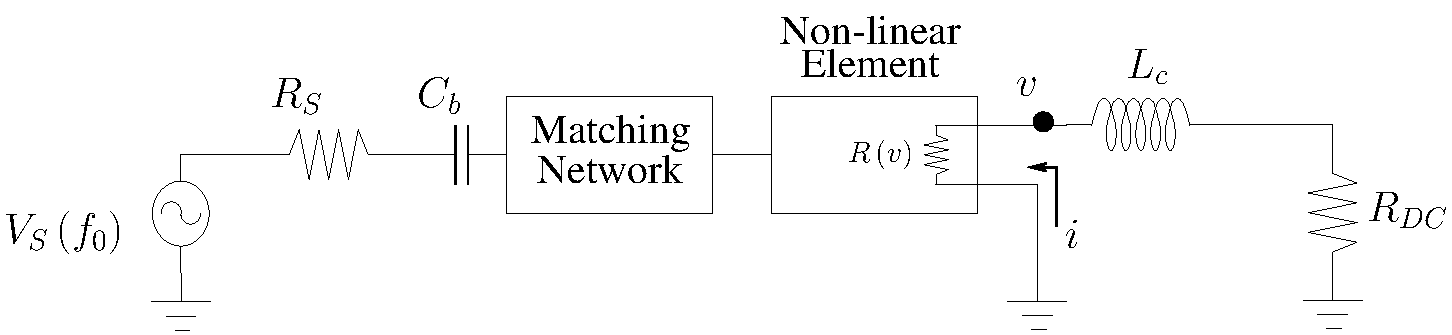
\includegraphics[width=3.5in]{pdf/01.pdf}\\
  \caption{Microwave rectifier circuit diagram. An ideal blocking capacitor $C_b$ provides DC isolation between the microwave source and rectifying element.  An ideal choke inductor $L_c$ isolates the DC load $R_{DC}$ from RF power.}\label{circuit_diagram}
  \end{center}
\end{figure}

The implementation was based on the file \textit{particle swarm optimization}. The essence is on \textit{ParticleSwarmOptimization} Class and \textit{Particle} Class development. The first one provides the interface in which the simulation communicates with the PSO.

Based on this, the development of \textit{ParticleSwarmOptimization} Class was oriented on receive inputs, provides information, and have methods that triggers the algorithm continuation.

In order to achieve this, it was developed the methods shown from the Code \ref{code:particle_swarm_optimization} to the Code \ref{code:notify_evaluation}.

\lstinputlisting[
    language=python,
    caption={Constructor of \textit{PSO} Class.},
    label={code:particle_swarm_optimization},
    style=cStyle,
    firstline=78,
    lastline=85
]{./../code/particle_swarm_optimization.py}

\lstinputlisting[
    language=python,
    caption={Method \textit{get best position} of \textit{PSO} Class.},
    label={code:get_best_position},
    style=cStyle,
    firstline=93,
    lastline=94
]{./../code/particle_swarm_optimization.py}

\lstinputlisting[
    language=python,
    caption={Method \textit{get best value} of \textit{PSO} Class.},
    label={code:get_best_value},
    style=cStyle,
    firstline=101,
    lastline=101
]{./../code/particle_swarm_optimization.py}

\lstinputlisting[
    language=python,
    caption={Method \textit{get position to evaluate} of \textit{PSO} Class.},
    label={code:get_position_to_evaluate},
    style=cStyle,
    firstline=110,
    lastline=111
]{./../code/particle_swarm_optimization.py}

\lstinputlisting[
    language=python,
    caption={Method \textit{advance generation} of \textit{PSO} Class.},
    label={code:advance_generation},
    style=cStyle,
    firstline=117,
    lastline=120
]{./../code/particle_swarm_optimization.py}

\lstinputlisting[
    language=python,
    caption={Method \textit{notify evaluation} of \textit{PSO} Class.},
    label={code:notify_evaluation},
    style=cStyle,
    firstline=129,
    lastline=141
]{./../code/particle_swarm_optimization.py}

The two main methods during the execution are \textit{get position to evaluate} that returns to simulation the position of on particle, and the \textit{nofify evalutation} that gives the simuation result of that position to the \textit{PSO} algorithm. With the result the code check if it is the best of that specific particle, or if it is the best overall. Then advance the index to next iteration.

This advance index step is quite important, bacause if the index reaches the population size, it calls the method \textit{advance generation} that will update the velocity and the position of every particle and reset the index.

\subsection {Particle Class Implementation}

Objects of this class stores its position, its velocity, and its best position. The class provides, as well, methods to the particle update its velocity and its position.

The implementation of Particle Class is shown from Code \ref{code:particle} to Code \ref{code:update_particle_position}.

\lstinputlisting[
    language=python,
    caption={Constructor of \textit{Particle} Class.},
    label={code:particle},
    style=cStyle,
    firstline=19,
    lastline=41
]{./../code/particle_swarm_optimization.py}

\lstinputlisting[
    language=python,
    caption={Method \textit{update particle velocity} of \textit{PSO} Class.},
    label={code:update_particle_velocity},
    style=cStyle,
    firstline=43,
    lastline=51
]{./../code/particle_swarm_optimization.py}

\lstinputlisting[
    language=python,
    caption={Method \textit{update particle position} of \textit{PSO} Class.},
    label={code:update_particle_position},
    style=cStyle,
    firstline=53,
    lastline=59
]{./../code/particle_swarm_optimization.py}

\subsubsection{Update velocity}

The \texit{updatae velocity} method uses Equation \ref{equation:update_velocity}. Where $r_p$ and $r_g$ are two different random numbers between 0 and 1 generated on every time the equation is calculated.

The $\phi_p$ is called the congnitve parameter, and it is a constant that multiplies the vector $(b_i - x_i)$ which is the direction to the best position of that particle.

The $\phi_g$ is called the social parameter, and it is a constant that multiplies the vector $(b_g - x_i)$ which is the direction to the best position in all particles.

Therefore the constants $\phi_p$ and $\phi_g$ balance how much important will be the best position locally and the best position globally.

Basicly this is a balance between explorateion and explotation. The bigger the importancy of the global best, the more proprable to converge to a not so good local maximum. The bigger the importancy of local best, the more problable to find a better solution, but with a more slow convergency.

\begin{equation}
    \label{equation:update_velocity}
    v_{i+1} = \omega v_i + \phi_p r_p (b_i - x_i) + \phi_g r_g (b_g - x_i)
\end{equation}

\subsubsection {Update position}

In order to update the particle position. Its current position is added to its calculated new velocity. This can is seen in the Code \ref{code:update_particle_position}.

As professor Maximo suggested during his lecture, it was implemented a particle reflection, when one of them fall out of the bounderies while updating its position.

\section{PSO result in test function}

As suggested, the PSO implementation was fist tested using an easy test function in order to verify its correctness.

The cost function used in the test was described on Equation \ref{equation:test_fuction}, in which has a global maximum $[1 2 3]$.

\begin{equation}
    \label{equation:test_fuction}
    f(x, y, z) = -((x - 1)^2 + (y-2)^2 + (z-3)^2)
\end{equation}

In tests conducted usin 40 particles and 1000 generations, the PSO converged rapdly to the global maximum. The position an quality of the results can be seen in Code \ref{code:position_test_function} and Code \ref{code:quality_test_function}.

\lstinputlisting[
    language=python,
    caption={Positions results on Test function, shown only the first 10 and the last 10.},
    label={code:position_test_function},
    style=cStyle,
]{./../code/test_function_result/test_short_position_history.txt}

\lstinputlisting[
    language=python,
    caption={Quality result on Test function, shown only the first 10 and the last 10},
    label={code:quality_test_function},
    style=cStyle,
]{./../code/test_function_result/test_short_quality_history.txt}

It is possible to see with the Figure \ref{img:test_best_quality_converge} to Figure \ref{img:test_parameters_quality_converge}, the convergency on the best position, the overall converge, and the converge of the parameters.

\begin{figure}
  \begin{center}
  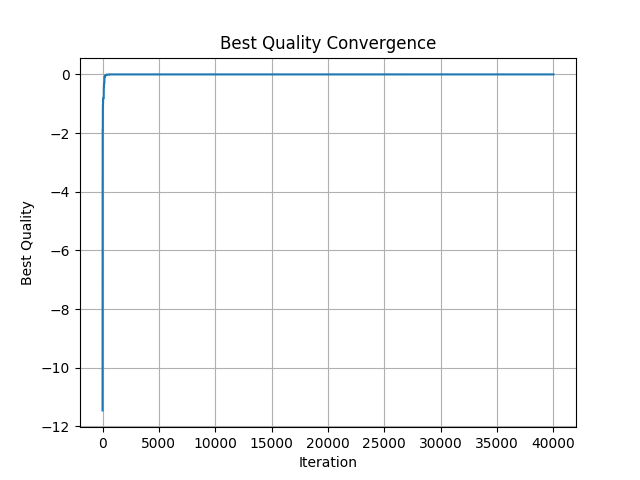
\includegraphics[width=2.8in]{./../code/test_function_result/test_best_convergence.png}
  %\vspace{-15pt}
  \caption{Test best quality convergency}
  \label{img:test_best_quality_converge}
  \end{center}
\end{figure}

\begin{figure}
  \begin{center}
  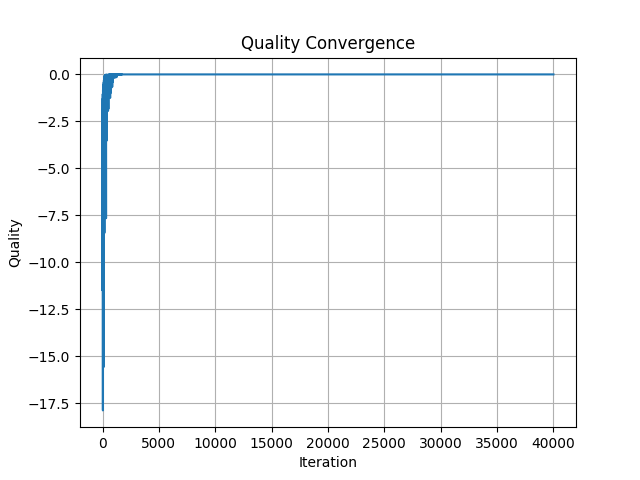
\includegraphics[width=2.8in]{./../code/test_function_result/test_quality_converge.png}
  %\vspace{-15pt}
  \caption{Test quality convergency}
  \label{img:test_quality_converge}
  \end{center}
\end{figure}

\begin{figure}
  \begin{center}
  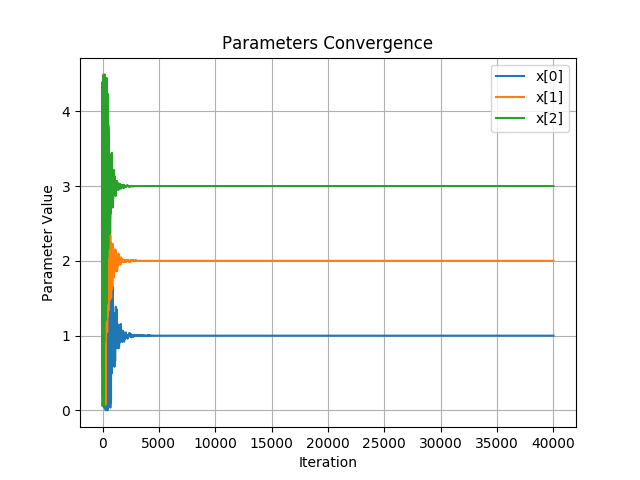
\includegraphics[width=2.8in]{./../code/test_function_result/test_parameters_converge.png}
  %\vspace{-15pt}
  \caption{Test parameters convergency}
  \label{img:test_parameters_quality_converge}
  \end{center}
\end{figure}

Thus it is clear that the algorithm works and converges accordingly. That said, the algorithm is ready to be used on the line follower problem.

\section {PSO on Line Follower Problem}

From a car circuit simulation, it was developed a line follower opmization on the \textit{proportional–integral–derivative controller (PID controller)} Control technique.

From the Equation \ref{equation:control_equation}, the objectve of this optimization is to optimize $K_p$, $K_i$, $K_d$, and the linear velocity of the car.

\begin{equation}
    \label{equation:control_equation}
    u(t) =  K_p e(t) + K_i \int_{0}^{t} e(t')dt'+K_d \frac{de(t)}{dt}
\end{equation}

In oder to do that, the \textit{PSO} algorithm was runned with 40 particles and it was developed the \textit{evaluate} method. With this method every positon of the car were evaluated and the sum of all evaluations was the score of the position of that particle.

The \textit{evaluate} method can be seen in the Code \ref{code:evaluate}, where by the end of the implementation was defined a high weight on linear speed and severe penalty for high errors and miss the track.

\lstinputlisting[
    language=python,
    caption={Method \textit{evaluate} of \textit{Simulation} Class, it is intended atribute a score for the situation of a particle.},
    label={code:evaluate},
    style=cStyle,
    firstline=130,
    lastline=152
]{./../code/simulation.py}

\subsection{Initials Tests}

In the firsts tests, it was clear that the convergency was always slow and always tending first to a quite slow velocity.

Therefore a higher weight was given to linear speed and 












Consider the microwave rectifier shown in Fig.~\ref{circuit_diagram}.  A sinusoidal microwave power source with voltage magnitude $V_s$ and impedance $R_s$ drives the rectifying element having a resistance $R(v)$ defined as
\begin{equation}\label{ideal_rectifier_resistance}
R(v) =
\begin{cases}
    \infty, & v > 0\\
    0, & v \leq 0
\end{cases}
\end{equation}
where $v$ and $i$ are the instantaneous voltage across and current through the rectifying element, respectively. The rectifying element depicted by $R(v)$ in Fig.~\ref{circuit_diagram} can in general be any nonlinear device that acts as a switch, such as a diode or a transistor. When a non-zero on-resistance $R_{on}$ and non-zero threshold voltage $V_{tr}$ are taken into account, the resistance of the rectifying element is given by

\begin{equation}\label{nonideal_rectifier_resistance}
R(v) =
\begin{cases}
    \infty, & v > -V_{tr}\\
    R_{on}, & v \leq -V_{tr}
\end{cases}
\end{equation}

The analysis of different classes of power rectifiers will next be analyzed based on the harmonic terminations presented to the rectifying element, and independent of the physical nonlinear device which performs the rectification.









\subsection {Class-C Rectifier Analysis}

In Fig.~\ref{circuit_diagram}, a sinusoidal microwave power source with voltage magnitude $V_s$ and impedance $R_s$ drives the rectifying element of resistance $R(v)$ above. The DC load seen by the rectifying element is $R_{DC}$ while the load at the fundamental frequency $f_0$ and successive harmonics is set by the matching network. Assume the matching circuit presents $R_s(f_0)$ to the rectifying element with all subsequent harmonics terminated in short circuits. This is equivalent to the harmonic terminations for a canonical reduced conduction angle power amplifier. This class is useful for Schottky diode rectifiers because these diodes have nonlinear junction capacitance. Short-circuiting the harmonics fixes the harmonic terminations at the intrinsic diode by shorting this junction capacitance.

When the incident RF voltage at the ideal rectifier swings negative, it is clipped at zero given (\ref{ideal_rectifier_resistance}).  The enforced harmonic terminations force the voltage waveform to contain only a DC and fundamental frequency component. Therefore, a DC component must be produced by the rectifying element such that the voltage waveform maintains its sinusoidal nature.  The voltage across the rectifying element can now be expressed as

\begin{equation}\label{diode_voltage_waveform_B}
    v(\theta) = V_{DC} + V(f_0)\sin(\theta)
\end{equation}
where $V(f_0)$ is the fundamental frequency component of the voltage across the rectifying element, $V_{DC}$ is the DC component, $V_{DC} = V(f_0)$ and $\theta = 2\pi f_0 t$. The current waveform contains infinite frequency components, and can be written as

\begin{equation}\label{diode_current_waveform_time_domain}
    i(\theta) = 2\pi I_{DC}\delta\left(\theta-\frac{3\pi}{2} - 2n\pi\right), \hskip 1pc n = 0,1,...,\infty
\end{equation}
where $I_{DC}$ is the DC current and $\delta(\theta)$ is the Dirac delta function. When all available input power $P_{in}$ is delivered to the rectifier, the fundamental frequency component of the current through the rectifying element $I(f_0)$ is
\begin{equation}\label{diode_current_waveform_finv_fo}
I(f_0) = \frac{2P_{in}}{V(f_0)}
\end{equation}
and, since there is no mechanism by which the rectifier itself can dissipate power ($R_{on}=0$ at this point), all of the available input power must be dissipated in the DC load and the conversion efficiency is 100\%. Therefore,

\begin{equation}\label{dcload}
P_{in} = V_{DC}I_{DC}
\end{equation}

Substituting in \hl{(}\ref{diode_current_waveform_finv_fo}\hl{)} and rearranging gives the expression of the current at the fundamental input frequency and the DC rectified current, which is $I(f_0) = 2I_{DC}$. When all available input power is delivered to the rectifier, the RF-DC conversion efficiency is 100\% because the rectifying element is ideal and cannot dissipate power itself.  In order for all available input power to be delivered to the rectifier, it is straightforward to show that the DC load must be set relative to the fundamental frequency load as
\begin{equation}\label{ideal_DC_load}
R_{DC} = 2R_s(f_0)
\end{equation}

A harmonic balance simulation of an approximately ideal rectifier with short-circuited harmonic terminations was performed in Microwave Office$\textsuperscript{\textregistered}$ using the SPICE diode model with no parasitics (PNIV) as the rectifying element.  The device temperature was set to $1^\circ$\,K to approximate an ideal switch.  The fundamental frequency excitation was set to 1\,W at 1\,GHz with the first 200 harmonics terminated in short-circuits.  The diode was presented with 50\,$\Omega$ at the fundamental frequency and the DC load was swept from 5\,$\Omega$ to 200\,$\Omega$.  The simulated data is then normalized to generalize the simulation results. The ideal time-domain current and voltage waveforms across the diode are shown in Fig.~\ref{waveforms} with the RF-DC conversion efficiency as a function of $R_{DC} / R_s(f_0)$ for varying rectifier on-resistance shown in Fig.~\ref{sim_opt_eff}.  It is clear that the mechanism of operation in the ideal case agrees with the theory presented above.  The reduction in RF-DC conversion efficiency when the DC load is not set according to (\ref{ideal_DC_load}) is due to impedance mismatch, and is given by


\begin{equation}\label{eff_dc_load}
\eta = 1 - \left(\frac{R_{DC} - 2R_s(f_0)}{R_{DC} + 2R_s(f_0)}\right)^2
\end{equation}

% ==== FIG 2
\begin{figure}
  \begin{center}
  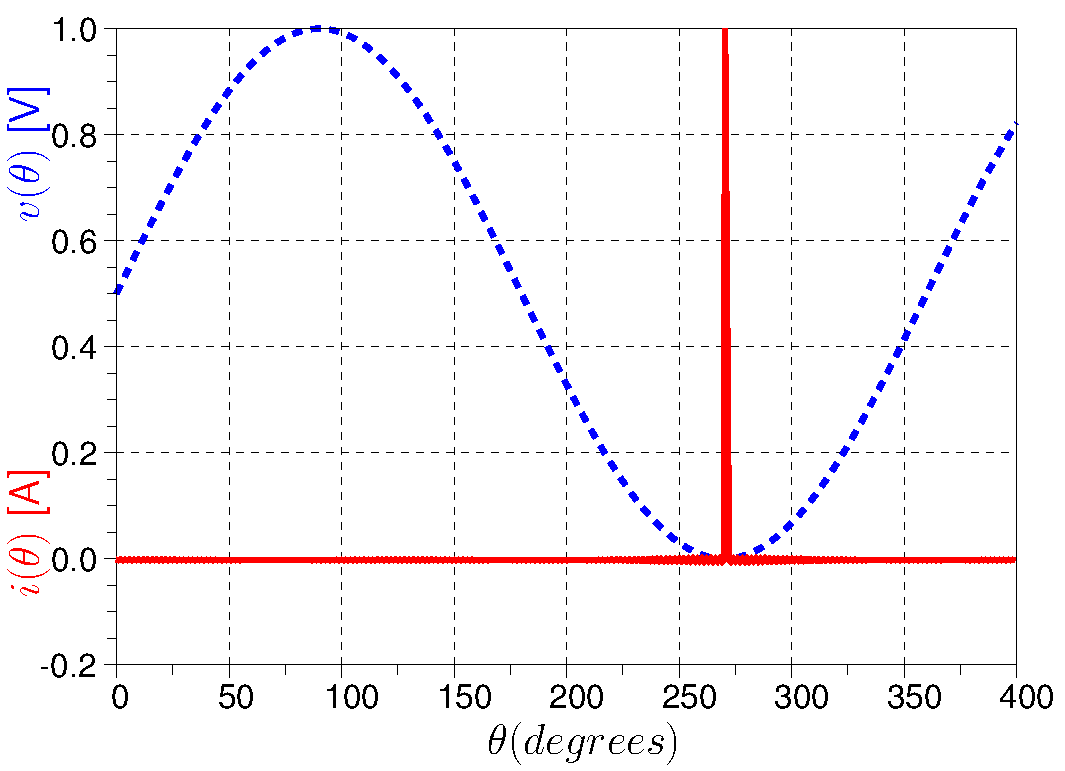
\includegraphics[width=2.8in]{pdf/02.pdf}
  %\vspace{-15pt}
  \caption{\hl{Ideal normalized voltage (dashed) and current (solid) waveforms for reduced conduction angle half-wave rectifier. The waveforms have been normalized to their peak values.}}\label{waveforms}
  \end{center}
\end{figure}

% ==== FIG 3
\begin{figure}
  \begin{center}
  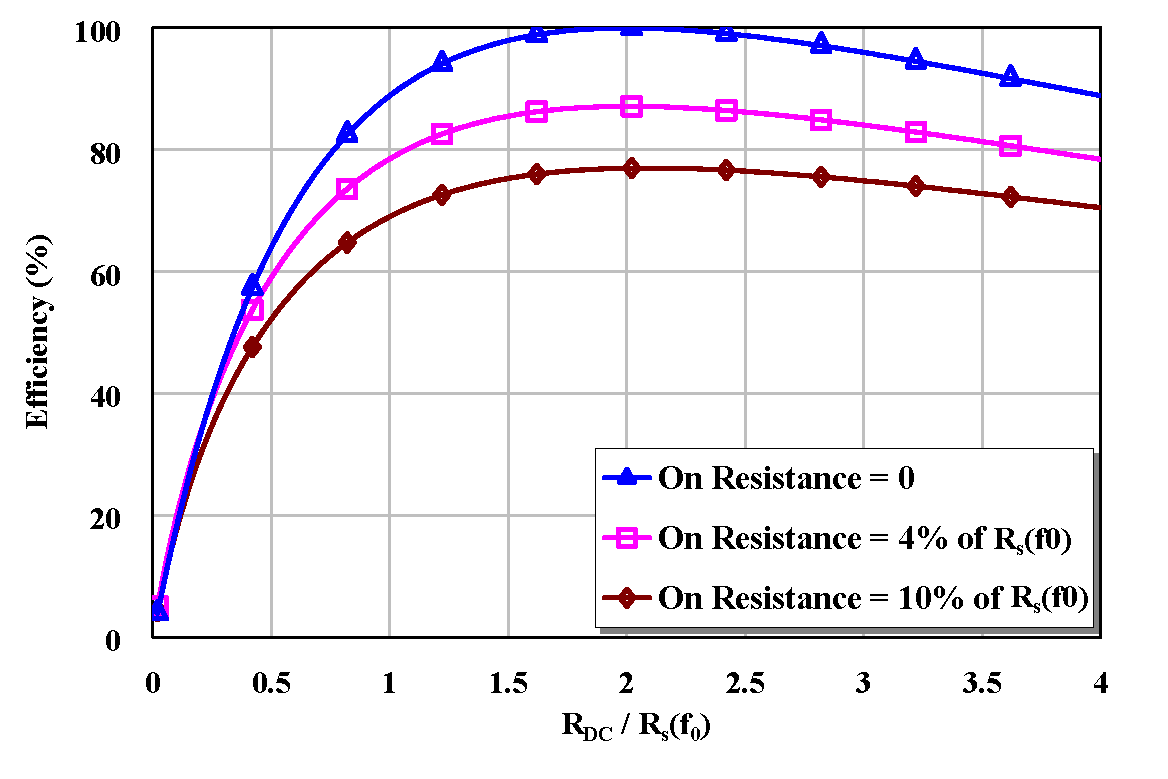
\includegraphics[width=3.5in]{pdf/03.pdf}
 % \vspace{-15pt}
  \caption{Simulated efficiency of reduced conduction angle half-wave rectifier versus $R_{DC} / R_s(f_0)$ for varying rectifier on-resistance.}\label{sim_opt_eff}
  \end{center}
\end{figure}










\subsection {Class-F$^{-1}$ Rectifier Analysis}

Consider again the rectifier circuit shown in Fig.~\ref{circuit_diagram} and assume that all even harmonics are terminated in open circuits, while all odd harmonics are terminated in short circuits. This set of harmonic terminations is the same as for a class-F$^{-1}$ amplifier, therefore this rectifier will be referred to as a class-F$^{-1}$ rectifier. The fundamental frequency component of the voltage across the rectifying device is given by
\begin{equation}\label{fundamental_diode_voltage}
    V(f_0) = V_s(f_0)
\end{equation}

During the second half of the RF cycle, it is evident from (\ref{ideal_rectifier_resistance}) that the voltage across the rectifying element must be zero.  This condition must be met through the addition of DC and only even harmonic voltage components, and therefore the voltage waveform is expressed as

\begin{equation}\label{diode_voltage_waveform_finv}
v(\theta) =
\begin{cases}
    2V(f_0)\sin\theta, & 0 \leq \theta < \pi\\
    0, & \pi \leq \theta < 2\pi
\end{cases}
\end{equation}


A Fourier expansion of (\ref{diode_voltage_waveform_finv}) expresses the DC component of the voltage waveform as
\begin{equation}\label{DC_diode_voltage}
    V_{DC} = \frac{2V(f_0)}{\pi}
\end{equation}

In the first half of the RF cycle, the current through the rectifying element is zero, given (\ref{ideal_rectifier_resistance}). This condition is met through the addition of a DC current and odd harmonic current components. With the current direction as in Fig.~\ref{circuit_diagram}, the DC component of the current must be positive.  Therefore, in the first half of the RF cycle, the remaining harmonics must sum to a constant value equivalent to the negative of the DC component.  Since the function which is the sum of the remaining harmonics is odd, the second half of the RF cycle must sum to the DC component, and the current is given by
\begin{equation}\label{diode_current_waveform_finv}
i(\theta) =
\begin{cases}
    0, & 0 \leq \theta < \pi\\
    2I_{DC}, & \pi \leq \theta < 2\pi
\end{cases}
\end{equation}
The DC component of the current waveform Fourier expansion is found to be
\begin{equation}\label{DC_diode_current}
    I_{DC} = \frac{\pi}{4}I(f_0)
\end{equation}
The DC load consistent with (\ref{diode_voltage_waveform_finv}) and (\ref{diode_current_waveform_finv}) is given by
\begin{equation}\label{DC_resistance}
    R_{DC} = \frac{8V(f_0)}{\pi^2I(f_0)} = \frac{8}{\pi^2}R(f_0)
\end{equation}

The conversion efficiency, defined as the ratio of the DC power dissipated in the load resistor to the available fundamental frequency RF power, is evaluated as

\begin{equation}\label{eff_finv}
    \eta = \frac{P_{DC}}{P(f_0)} = \frac{2V_{DC}I_{DC}}{V(f_0)I(f_0)} = \frac{2\frac{2}{\pi}V(f_0)\frac{\pi}{4}I(f_0)}{V(f_0)I(f_0)} = 1
\end{equation}

Therefore, the ideal half-wave rectifier converts all available RF power to DC power if the the DC loading resistance set to the value given in (\ref{DC_resistance}). The RF-DC conversion efficiency as a function of $R_{DC} / R_s(f_0)$ was simulated in Microwave Office$\textsuperscript{\textregistered}$ for varying rectifier on-resistance and is shown in Fig.~\ref{sim_opt_eff_classFinv}. The harmonic balance settings were identical to those used for the class-C rectifier above. The peak efficiency as a function of on-resistance is higher than for the class-C rectifier, although the efficiency degrades more quickly when the non-ideal DC load is applied.

%For zero on-resistance, the optimal DC load is exactly that predicted by (\ref{DC_resistance}).
%The reason for the increase in optimal DC load as the on-resistance increases is that the current
%through the on-resistance is reduced, thus reducing the loss.  However, there is a penalty paid in
%reflected power from the rectifying element due to the non-ideal match.  This limits the benefit of
%increasing the DC load infinitely with a fixed fundamental frequency match.  Theoretically, if the
%fundamental and DC loads could be increased infinitely the efficiency would approach 100\,\% no matter
%how large the on-resistance became.
%
% SHOULD WE MAYBE MOVE THIS TO DISCUSSION OR POSSIBLY DELETE?

% ==== FIG 4
\begin{figure}[!b]
  \begin{center}
  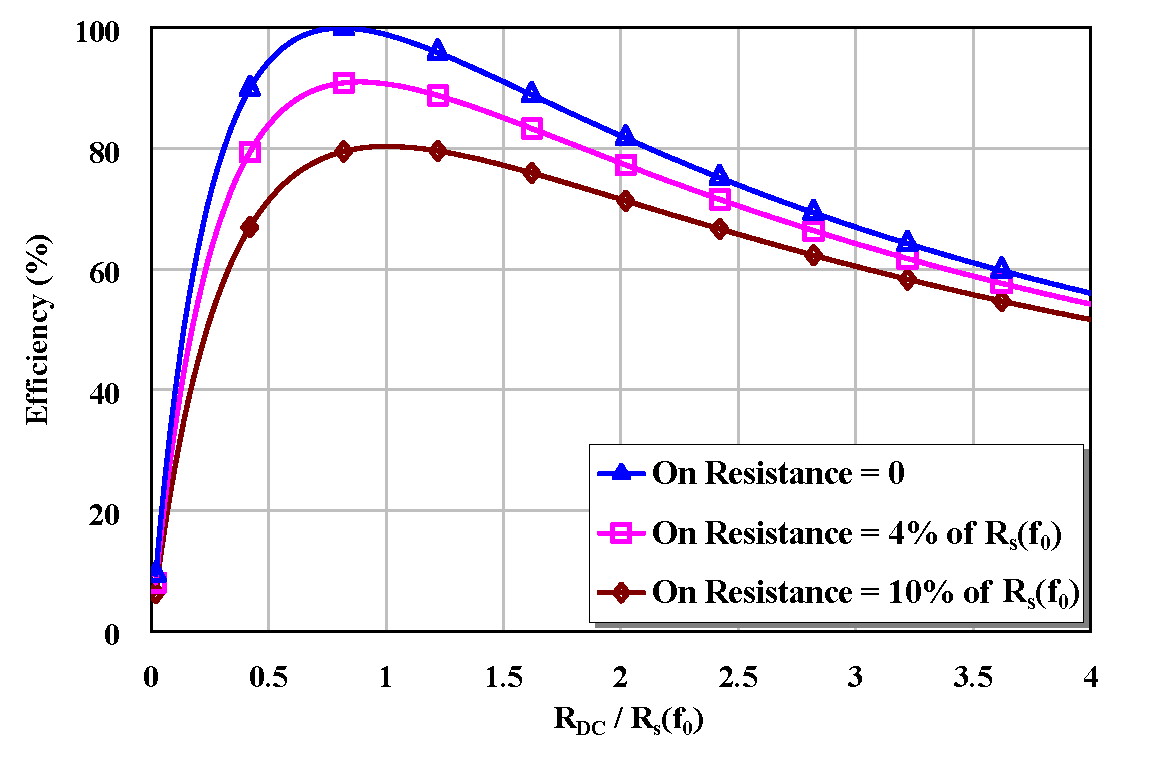
\includegraphics[width=3.5in]{pdf/04.pdf}
  %  \vspace{-15pt}
  \caption{Simulated efficiency of class-F$^{-1}$ rectifier versus $R_{DC} / R_s(f_0)$ for varying rectifier on-resistance.}\label{sim_opt_eff_classFinv}
  \end{center}
\end{figure}

The waveforms including parasitic on-resistance and threshold voltage are next investigated assuming the rectifier impedance from (\ref{nonideal_rectifier_resistance}). The time domain voltage and current waveforms are approximated as
\begin{equation}\label{diode_voltage_waveform_finv_par}
v(\theta) =
\begin{cases}
    V_{max}\sin\theta, & v(\theta) > -V_{tr}\\
    -V_{tr} - I_{max}R_{on}, & v(\theta) \leq -V_{tr}
\end{cases}
\end{equation}
\begin{equation}\label{diode_current_waveform_finv_par}
i(\theta) =
\begin{cases}
    0, & V(\theta) > -V_{tr}\\
    I_{max}, & v(\theta) \leq -V_{tr}
\end{cases}
\end{equation}



% === FIG 5
\begin{figure}[!b]
  \begin{center}
  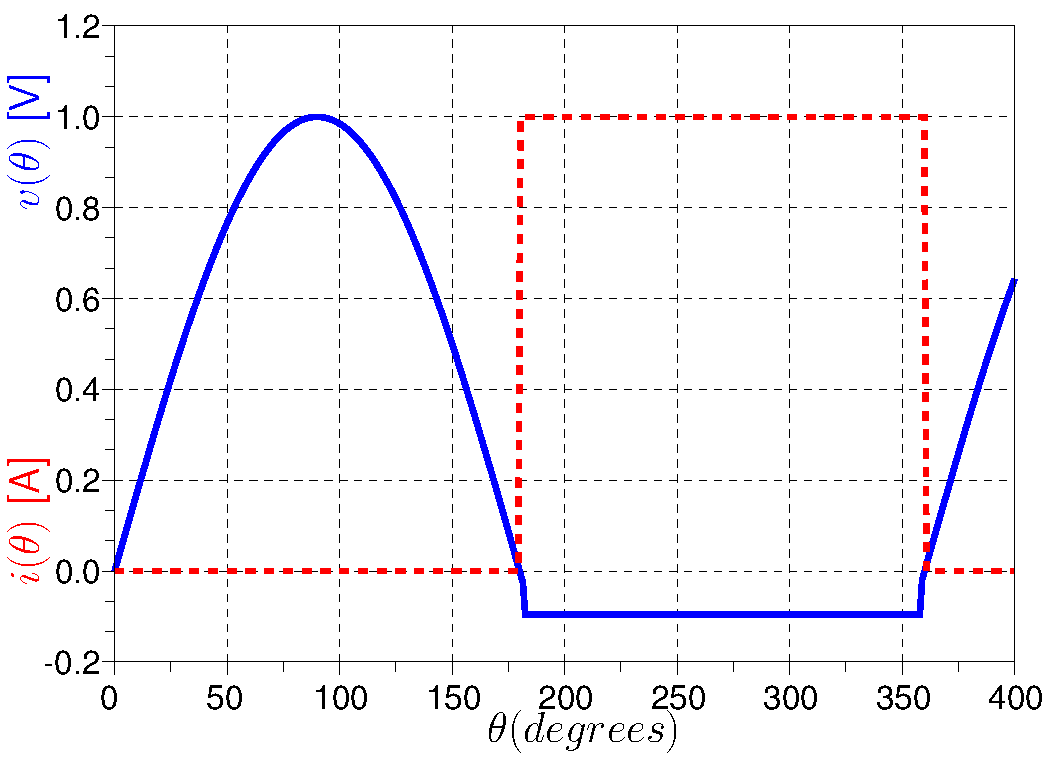
\includegraphics[width=3.0in]{pdf/05.pdf}
     % \vspace{-5pt}
  \caption{\hl{Non-ideal class-F$^{-1}$ voltage (solid) and current (dashed) waveforms, normalized to their peak respective values.}}\label{finv_waveform_nonideal}
  \end{center}
\end{figure}

As an example, Fig.~\ref{finv_waveform_nonideal} shows the current and voltage waveforms for a specific set of non-ideal parameters ($V_{tr} = 0.7\,\textrm{V}$, $V_{max} = 20\,\textrm{V}$, $I_{max} = 200\,\textrm{mA}$, and $R_{on} = 5\,\Omega$). When the device is conducting current, it creates a voltage drop across the on-resistance which is constant due to the constant current. If the on-resistance were zero, the only difference between the waveform in (\ref{diode_voltage_waveform_finv_par}) and the ideal voltage waveform would be the minimum value, which would be $-V_{tr}$ rather than zero. The values of $\theta$ at which the transition between the conducting and non-conducting regions occurs are found to be
\begin{equation}\label{trans_points_thetafinv2}
\begin{array}{l}
    \theta_{t1} = 2\pi - \arcsin\left(\frac{V_{tr}}{V_{max}}\right) \\
    \theta_{t2} = \pi + \arcsin\left(\frac{V_{tr}}{V_{max}}\right)
\end{array}
\end{equation}

The DC and fundamental frequency values of the voltage and current waveforms can be found through a Fourier analysis using the transition points in (\ref{trans_points_thetafinv2}). The first Fourier coefficient of $v(t)$ gives the DC component of the voltage, which can be derived as
\begin{equation}\label{finv_dc_comp_5}\begin{split}
    V_{DC} &= \frac{1}{2\pi}\left(2V_{max}\sqrt{1 - \left(\frac{V_{tr}}{V_{max}}\right)^2} \right. \\
    &-(V_{tr} + I_{max}R_{on})\left[\pi - 2\arcsin\left(\frac{V_{tr}}{V_{max}}\right)\right]\Bigg)
\end{split}\end{equation}

The fundamental frequency voltage is found from $V(f_0)=a_v+jb_v$, where
\begin{shaded}
\begin{equation}
a_v=\frac{1}{\pi}\int_0^{2\pi}v(\theta)\cos \theta d\theta = 0
\end{equation}
\end{shaded}
and $b_v$ can be reduced to


\begin{equation}\label{finv_vf0_comp_5}\begin{split}
    b_v =& \frac{1}{\pi}\Bigg(V_{max}\arcsin\left(\frac{V_{tr}}{V_{max}}\right)+ \frac{\pi V_{max}}{2}  \\
    &+ \left.\left(V_{tr} + 2I_{max}R_{on}\right) \sqrt{1 - \left(\frac{V_{tr}}{V_{max}}\right)^2}\right)
\end{split}\end{equation}

Similarly, the DC component of the current waveform is found to be

\begin{equation}\label{finv_idc_comp_3}
    I_{DC} = \frac{I_{max}}{2\pi}\left(\pi - 2\arcsin\left(\frac{V_{tr}}{V_{max}}\right)\right)
\end{equation}
The fundamental frequency current $i(t)=a_i+jb_i$ has $a_i=0$ and the coefficient $b_i$ can be shown to be equal to

\begin{equation}\label{finv_if0_comp_2}
    b_i = -\frac{2I_{max}}{\pi}\sqrt{1 - \left(\frac{V_{tr}}{V_{max}}\right)^2}
\end{equation}
The input power \hl{at the fundamental frequency} is found from


\begin{equation}\label{Pin}
  P_{in} = \Re\left\{\frac{V(f_0)I^{*}(f_0)}{2}\right\}
\end{equation}


\hl{Substituting (}\ref{finv_vf0_comp_5}) and (\ref{finv_if0_comp_2}) into the above results in

\begin{shaded}
\begin{equation}\begin{split}\label{Pin_diode2}
    P_{in} =& \frac{kI_{max}}{\pi^2}\left(V_{max}\arcsin\left(\frac{V_{tr}}{V_{max}}\right) + \frac{\pi V_{max}}{2} \right. \\
   &+ \left(V_{tr}+2I_{max}R_{on}\right)k\bigg)
\end{split}\end{equation}
\end{shaded}
where $k$ is defined as
\begin{equation}\label{k}
    k = \sqrt{1 - \left(\frac{V_{tr}}{V_{max}}\right)^2}
\end{equation}

Solving for $I_{max}$ as a function of $P_{in}$ when $R_{on}$ is non-zero after some arithmetic results in two solutions, one of which is negative. The positive solution for the maximal current is

\begin{equation}\label{Imax_solved1}
    I_{max} = \frac{ \sqrt{\alpha^2 + 8\pi^2P_{in}R_{on}}-\alpha}{4R_{on}k}
\end{equation}
with $\alpha=V_{max}\left(\arcsin\left(\frac{V_{tr}}{V_{max}}\right)+ \frac{\pi}{2} + k\frac{V_{tr}}{V_{max}}\right)$.

In the case where $R_{on}$ is zero, (\ref{Imax_solved1}) simplifies to
\begin{equation}\label{Imax_solve_zeroron_solved}
    I_{max} = P_{in}\frac{\pi^2}{kV_{max}\left(\arcsin\left(\frac{V_{tr}}{V_{max}}\right)+ \frac{\pi}{2} + k\frac{V_{tr}}{V_{max}}\right)}
\end{equation}

Note that in the case of an ideal rectifying element, $k = 1$ and $V_{tr} = 0$, therefore
\begin{equation}\label{Imax_solve_zeroron_solved_ideal}
    I_{max,ideal} = \frac{2\pi P_{in}}{V_{max}}
\end{equation}

Now that $I_{max}$ is fully expressed given known rectifier parameters, $V_{DC}$ and $I_{DC}$, $V(f_0)$ and $I(f_0)$ may be calculated, and from this, the DC load and the load at fundamental frequency determined from the following expressions:

\begin{equation}\label{rdcf}
    R_{DC} = \frac{V_{DC}}{I_{DC}}
\end{equation}

\begin{equation}\label{rf0f}
    R(f_0) = -\frac{V(f_0)}{I(f_0)} = -\frac{b_v}{b_i}
\end{equation}
The negative impedance in (\ref{rf0f}) indicates that power is delivered to the rectifying element and gives the impedance of the source delivering power to the rectifying element.  The rectifier efficiency is given by
\begin{equation}\label{efff}
    \eta = \frac{P_{DC}}{P_{in}} = \frac{V_{DC}I_{DC}}{P_{in}}
\end{equation}










\subsection {Design example based on class-F$^{-1}$ theory}

To understand the usefulness of the presented theory, assume the rectifying element has the following parameters: $V_{max} = 10$\,V, $R_{on} = 5$\,$\Omega$, $V_{tr} = 0.7$\,V and $P(f_0)$ = 1\,W.  First, (\ref{Imax_solved1}) is used to calculate $I_{max}=456.7$\,mA. Next, the DC voltage and current are evaluated using (\ref{finv_dc_comp_5}) and (\ref{finv_idc_comp_3}), respectively, to give $V_{DC}=1.75$\,V and $I_{DC}=218.2$\,mA. The fundamental frequency voltage and current Fourier coefficients are then calculated to be $V(f_0)=6.896$\,V and $I(f_0)=-290$\,mA, respectively.  The DC and fundamental frequency resistances are then calculated using (\ref{rdcf}) and (\ref{rf0f}) to be $R_{DC}=8.02$\,$\Omega$ and $R(f_0)=23.77$\,$\Omega$, respectively.  The efficiency is then calculated using (\ref{efff}) to be $\eta$ = 38.18\,\%. If the input power is selected as 0.1\,W rather than 1\,W, the resultant efficiency is 72.43\,\% instead.  A specific rectification device will always have an approximate input drive level at which it can be most efficient, just as with power transistors in power amplifiers. To maximize efficiency, the goal is always to minimize the amount of power dissipation in the on-resistance of the rectifying element and maximize the power dissipated in the DC load resistor.









% === III. Schottky-Diode Class-C Rectifier =======================================
% =================================================================================
\section{Schottky-Diode Class-C Rectifier}

The Skyworks SMS7630 Schottky diode in the SC-79 package was selected for the half-wave rectifier. Source-pull was performed at 2.45\,GHz with 0-10\,dBm available input power for various DC loads in order to identify the combination of input power, fundamental load and DC load resulting in highest efficiency.  The best case occurred at 6\,dBm input power, with the source-pull contours being shown in Fig.~\ref{lpcontours}.  The on-resistance of the SMS7630 is 20\,$\Omega$ with the optimal DC load of 1080\,$\Omega$. Therefore $R_{on}$ is approximately 2\% of $R_{DC}$\hl{,} which in theory is 4\% of $R_s(f_0)$.  From Fig.~\ref{sim_opt_eff}, a peak efficiency of 87\% occurs with infinite harmonic terminations, therefore the achieved 77.6\% is very reasonable considering only the 2$^{\rm nd}$ and 3$^{\rm rd}$ harmonics were explicitly terminated.



\begin{figure}
  \begin{center}
  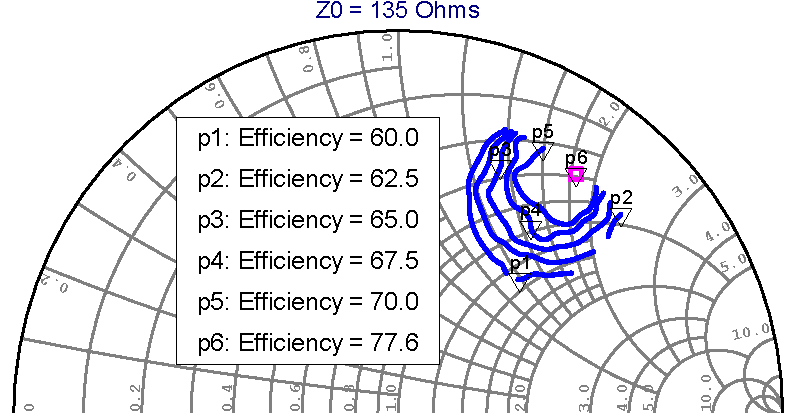
\includegraphics[width=3.0in]{pdf/06.pdf}\\
 \caption{\hl{Source-pull contours with available input power to the diode set to 6\,dBm.  The impedance is referenced to the junction capacitance of the diode, therefore the lead inductance of the package has been compensated for. Setting $R_{DC}$ to 1080\,$\Omega$ was found to result in the optimal efficiency for this input power. The highest efficiency of 77.6\% is obtained at $Z_{p6}=(68+j245)\Omega$ with $V_{DC}$=1.82\,V.}}\label{lpcontours}
  \end{center}
\end{figure}

%  \caption{Source-pull contours with available input power to the diode set to 6\,dBm.  The impedance is referenced to the junction capacitance of the diode, therefore the lead inductance of the package has been compensated for. Setting $R_{DC}$ to 1080\,$\Omega$ was found to result in the optimal efficiency for this input power.}\label{lpcontours}


\begin{figure}
  \begin{center}
  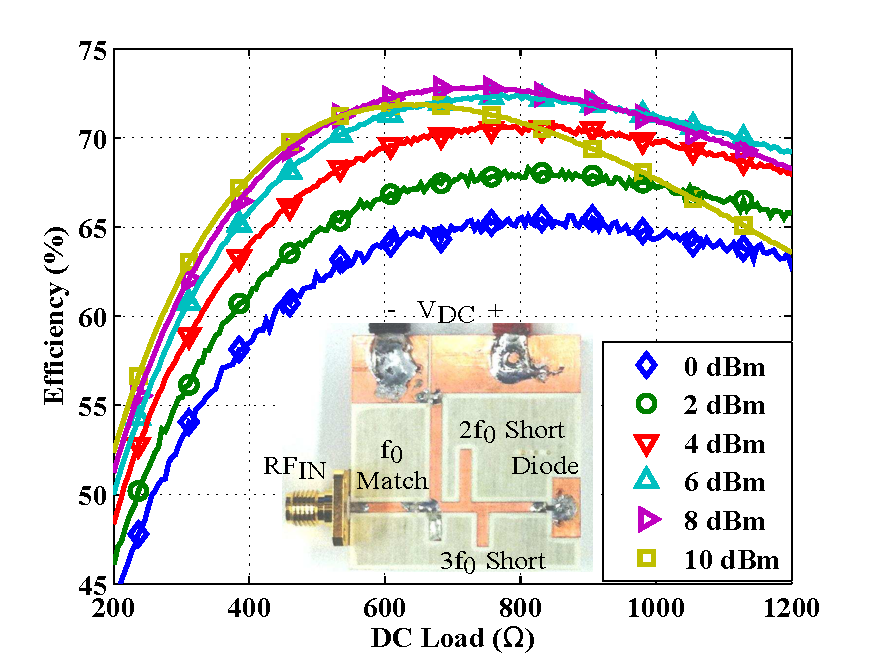
\includegraphics[width=3.5in]{pdf/07.pdf}\\
 \caption{\hl{RF-DC conversion efficiency versus DC load for fixed available input powers with 0.6\,dB matching network loss de-embedded.  The maximum efficiency of 72.8\% occurred at 8\,dBm with $R_{DC}$ = 742\,$\Omega$ and $V_{DC}$=1.91\,V, which is lower than the 1080\,$\Omega$ found during source-pull.  However, the efficiency at 1080\,$\Omega$ is 69.9\% which is very close to the peak value.}}\label{final_dc_sweep}
  \end{center}
\end{figure}

%  \caption{RF-DC conversion efficiency versus DC load fixed available input powers with 0.6\,dB matching network loss de-embedded.  The maximum efficiency of 72.8\% occurred at 8\,dBm with $R_{DC}$ = 742\,$\Omega$, which is lower than the 1080\,$\Omega$ found during source-pull.  However, the efficiency at 1080\,$\Omega$ is 69.9\% which is very close to the peak value.}\label{final_dc_sweep}


Measurements of a rectifier designed using the source-pull data show a maximum RF-DC conversion efficiency of 72.8\% when matched to 50$\Omega$, obtained after the 0.6\,dB matching network loss is de-embedded.  The fabricated rectifier and DC load sweep measurements are shown in Fig.~\ref{final_dc_sweep}. Open circuit shunt stubs are used to present short-circuit terminations at the second and third harmonic.  A shunt capacitor is used for presenting the fundamental frequency impedance to reduce size and allow tunability.  The reduction in efficiency relative to the source-pull measurements is due to the matching circuit not presenting the ideal impedance found during source-pull.





The class-C rectifier can be applied to improving the efficiency of a wireless powering reception device as demonstrated in \cite{robergIMS2012} with a dual-linearly polarized patch rectenna, with a rectifier circuit for each polarization. In this circuit, the first 5 harmonics are shorted and the impedances are validated by calibrated measurements and are presented in \cite{robergIMS2012}.















% === IV. Transistor Class-F inv Rectifier ========================================
% =================================================================================
\section{Transistor Class-F$^{-1}$ Rectifier}

To prove experimentally the duality between harmonically terminated PAs and rectifiers, a high-efficiency class-F$^{\rm -1}$ PA was designed, measured first as an amplifier, and then as a rectifier. In the rectifier measurements, RF power is input into the drain which is unbiased. The gate is terminated in a variable impedance and biased close to pinch-off. Measurements of efficiency and DC voltage are performed in time domain as a function of input RF power, gate RF load, gate bias and drain DC load.

\subsection {Circuit design}

A 2.14-GHz power amplifier, pictured on Fig.~\ref{amplifier}, is designed using the Triquint TGF2023-02 GaN pHEMT \cite{gan_pa_letter}. Class F$^{-1}$ harmonic terminations are implemented at the second and third harmonic. The performance of the PA, illustrated in  Fig.~\ref{PA_meas}, was characterized at 2.14\,GHz with a drain voltage bias of 28\,V and a bias current of 160\,mA. The PA exhibits a PAE of 84\% with an output power of 37.6\,dBm and a gain of 15.7\,dB under 3\,dB compression. The same PA design was used for rectifier measurements as shown in Fig.~\ref{measurement_setup}. \hl{The PA is connected to an input RF source at the drain, with the drain supply disconnected. The gate terminal is biased, and connected to an impedance tuner, converting the two-port transistor PA to a one-port rectifier, corresponding to the generalized schematic of Fig.}~\ref{circuit_diagram}.

% === FIG : Amplifier Picture
\begin{figure}[ht!]
\centering
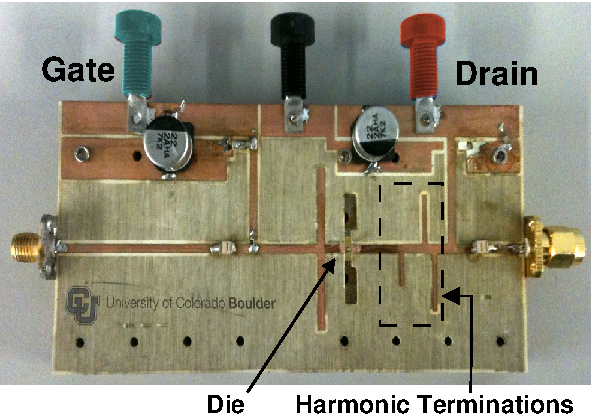
\includegraphics[width=3.0in]{pdf/08.pdf}
\caption{Photograph of the class-F$^{-1}$ power amplifier, working at 2.14 GHz and presented in \cite{gan_pa_letter}.}
\label{amplifier}
\end{figure}


% === FIG : PA measurements
\begin{figure}
  \begin{center}
  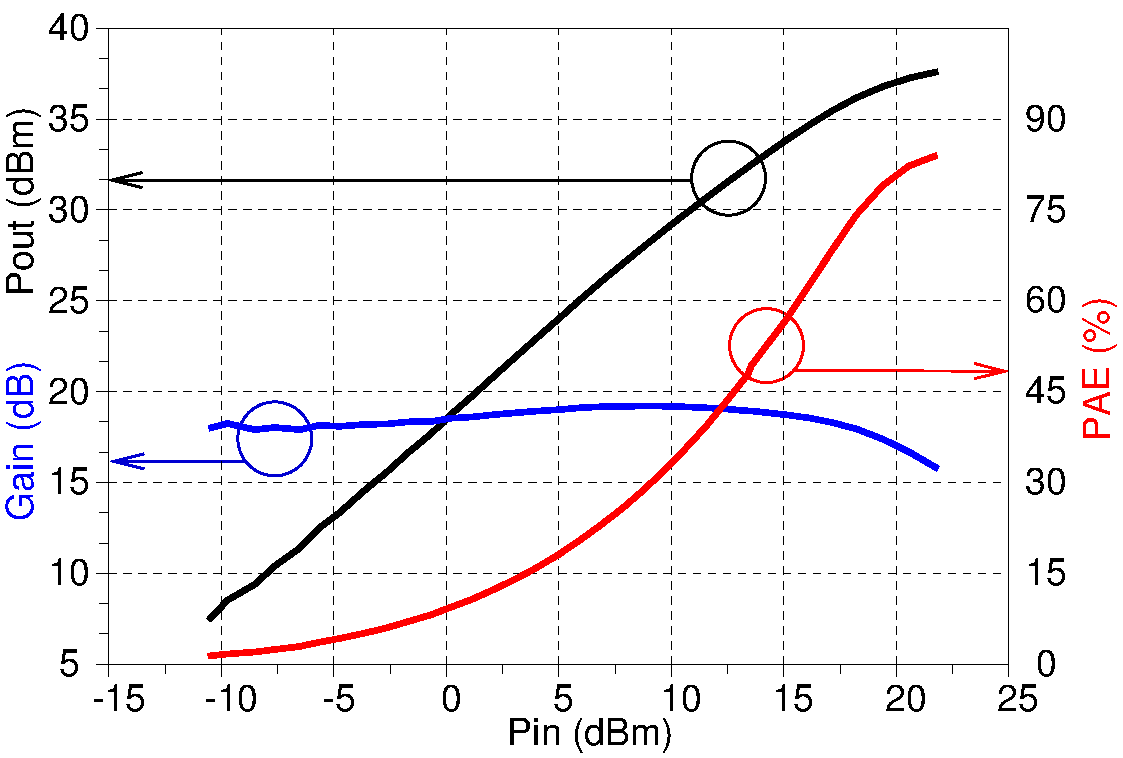
\includegraphics[width=3.0in]{pdf/09.pdf}
  \caption{\hl{Large-signal measurements performed on the class-F$^{-1}$ power amplifier at $f_0=2.14$\,GHz, $V_{GS}=-3.8$\,V and $V_{DS}=28$\,V}}
\label{PA_meas}
  \end{center}
\end{figure}









\subsection {Measurement setup}
%
The class-F$^{\rm -1}$ power amplifier described above is fully characterized in large signal in a rectifier configuration with the setup shown in Fig.~\ref{measurement_setup}. The commercial time-domain large signal measurement instrument is a VTD SWAP four-channel receiver \cite{SWAP}. In order to acquire time domain waveforms at the reference plane, an 8 error term model calibration similar to the one performed for LSNA \hl{(Large Signal Network Analyzer)} measurements is applied. After \hl{an absolute VNA-like calibration} \cite{verspecht}, the RF voltage and current waveforms at the input (V1 and I1) and at the output (V2 and I2) of the DUT are measured at the coaxial reference plane. In this case, the RF input is the drain port of the PA, while the RF output is connected to the gate port. Thus, performing a load pull on this device consists of varying the load at $f_0$ at the RF gate port of the PA with a passive tuner. This kind of measurement is similar to large signal characterization of switch devices recently reported in \cite{switch,faraj_arftg_2012}. The gate DC path is connected to a power supply so the gate bias can be varied. The drain DC bias is the output of the rectifier and is connected to a variable resistance $R_{DC}$, and the DC voltage across it is measured with a voltmeter. The DC current is then found from the value of $R_{DC}$ from (\ref{rdcf}). During the measurement, several parameters are varied systematically: the RF load impedance applied at the PA gate port $Z_g(f_0)=V_g(f_0)/I_g(f_0)$; the resistor in the DC drain output $R_{DC}$; and the gate bias voltage $V_{GS}$. The conversion efficiency of the rectifier and the DC power delivered at the drain output of the rectifier $P_{DC}= V_{DC} \cdot I_{DC}$ are measured as these parameters are varied, and as a function of input power at the drain port $P_{in}(f_0)$.





\begin{figure}[ht!]
\centering
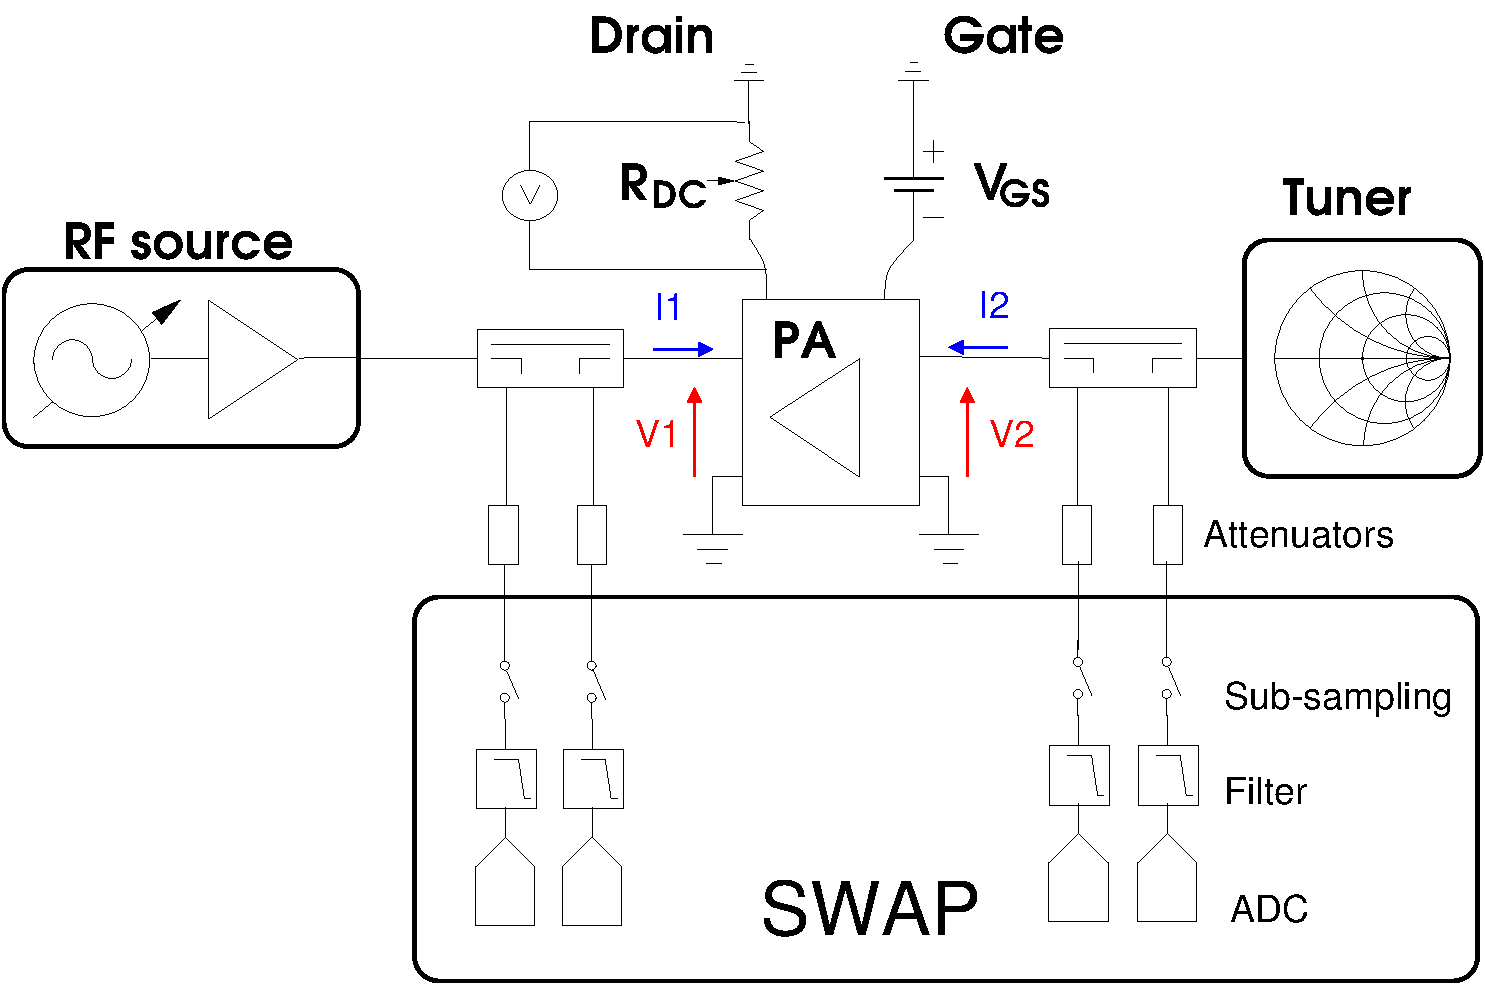
\includegraphics[width=3.5in]{pdf/10.pdf}
\caption{Time-domain non-linear rectifier measurement block diagram. The SWAP \cite{SWAP} performs sampling of current and voltage and the calibration refers the sampled quantities to the reference planes at the DUT. The drain output DC resistance $R_{DC}$ , the gate bias $V_{GS}$ and the gate RF impedance $Z_g$ are varied as the input power at the drain is swept from 10 to 42\,dBm.}
\label{measurement_setup}
\end{figure}














\subsection {Self-synchronous transistor rectifier results}

The measurements of the rectifier are performed in self-synchronous mode, i.e. there is no input RF power incident externally into the gate port of the PA, unlike in previous transistor rectifier work \cite{JoseIMS-rect,Kaz}. The following parameters are varied in order, while keeping the other parameters constant and sweeping the input RF power at the drain port, and the results are described in the same order:

\begin{enumerate}
\item RF impedance at the gate, $Z_g$;
\item load resistance at drain bias output, $R_{DC}$;
\item gate DC bias, $V_{GS}$.
\end{enumerate}

%\subsubsection{Sweeping \textbf{Tuner} - the RF load impedance at $f_0$ at the output (gate access)}
The gate load-pull was performed to determine the optimum impedance for maximum efficiency with a constant resistive DC load of 98.5\,$\Omega$ (nominally 100\,$\Omega$) and a constant transistor gate bias in pinch-off of -4.4\,V. The RF signal is coupled from the drain to the gate matching network through the feedback capacitance $C_{gd}$, and thus the precise impedance presented at the gate of the transistor is imperative to achieving high efficiency. Fig.~\ref{time-domain} shows the time-domain voltage and current waveforms measured at the drain and gate RF port of the amplifier when the RF input power at the drain port is swept from 11\,dBm to 42\,dBm. These values are chosen because the rectifier in PA operation gives up to 42\,dBm output power. The feedback signal present at the gate allows for the rectifier to operate in self-synchronous mode without any additional control signal. Unlike in the synchronously driven case where an external generator is connected to the gate, here the impedance presented at the gate is always passive (inside the Smith chart), keeping the device in a safe operating mode.

% === FIG : Time-domain waveforms
\begin{figure}[ht!]
\centering
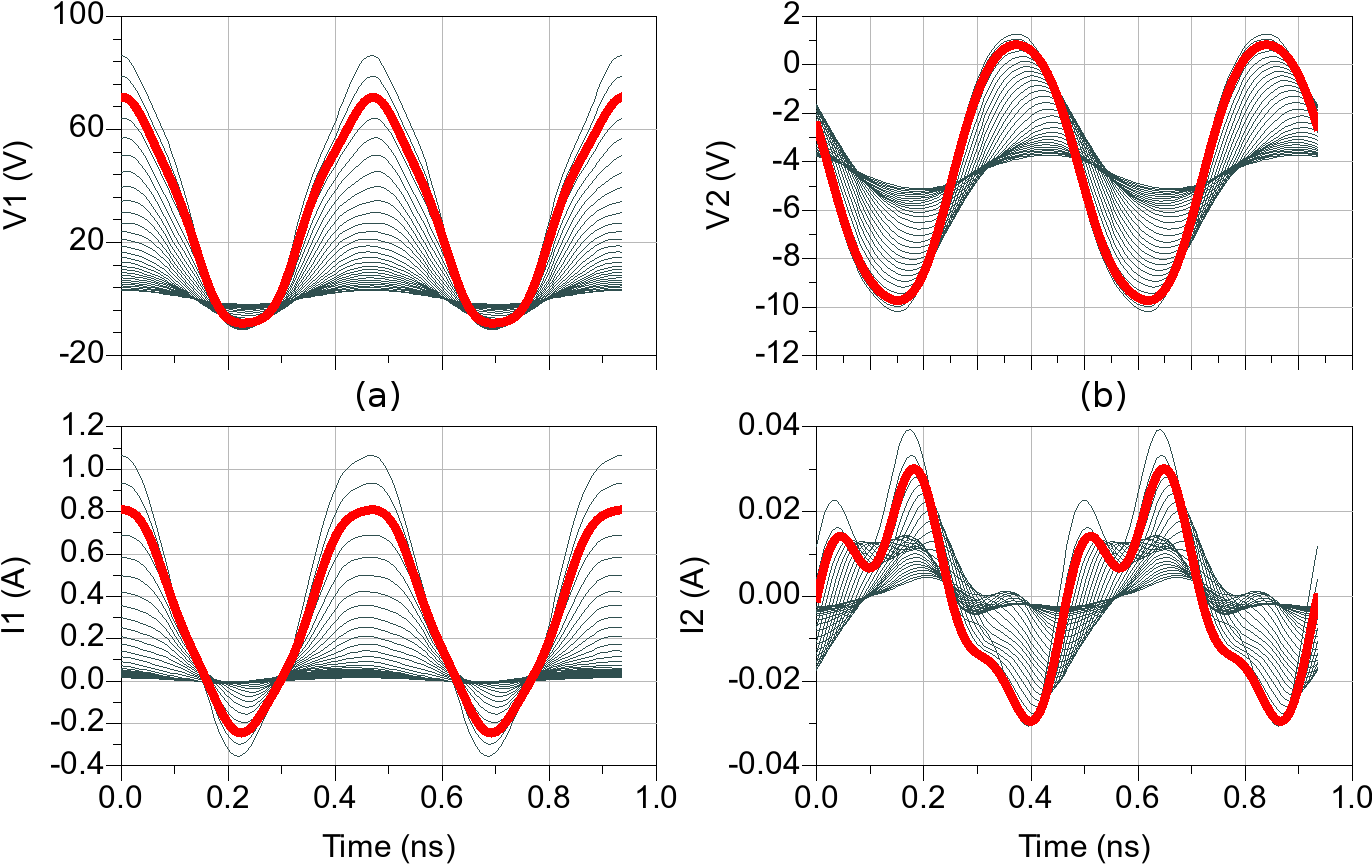
\includegraphics[width=3.4in]{pdf/11.png}
\caption{\hl{Time-domain waveforms measured at drain (a) and gate (b) of the rectifier with $V_{GS}=-4.4$\,V, $R_{DC}=98.5$\,$\Omega$ and $Z_g(f_0)=\left(230+j10\right)\Omega$. The RF input power at the drain is swept from 10 to 42\,dBm, corresponding to the range of output power of the class-F$^{-1}$ PA.}}
\label{time-domain}
\end{figure}

Measured RF-DC conversion efficiency is shown in Fig.~\ref{MEAS_LP_sweep} for four different RF gate impedances. A maximal conversion efficiency of 85\% is achieved with a DC output voltage of 36\,V and an input power at the drain of 42\,dBm \hl{with $R_{DC}=98.5\,\Omega$}. This peak efficiency is for a RF gate load of around 230\,$\Omega$ (green \hl{hexagon} in the Smith chart in Fig.~\ref{MEAS_LP_sweep}), which is the highest impedance that was achievable with the specific tuner in the setup. For the low gate impedance (red \hl{triangle} in the Smith chart), the efficiency is significantly lower. By observing the gate current (Fig.~\ref{MEAS_LP_sweep}d), it can be seen that for a low RF gate impedance, the gate diode turns on at around $P_{in}=25$\,dBm. Since the input power cannot be increased much beyond this point to avoid breakdown, this limits the DC voltage at the output to around 4\,V. For the gate impedance with highest efficiency (\hl{green line with hexagon symbol}), the gate diode is off for input drain powers below 41\,dBm, allowing for high DC voltage output.


%talk about Gate Idc ?




% === FIG : LP SWEEP
\begin{figure}[ht!]
\centering
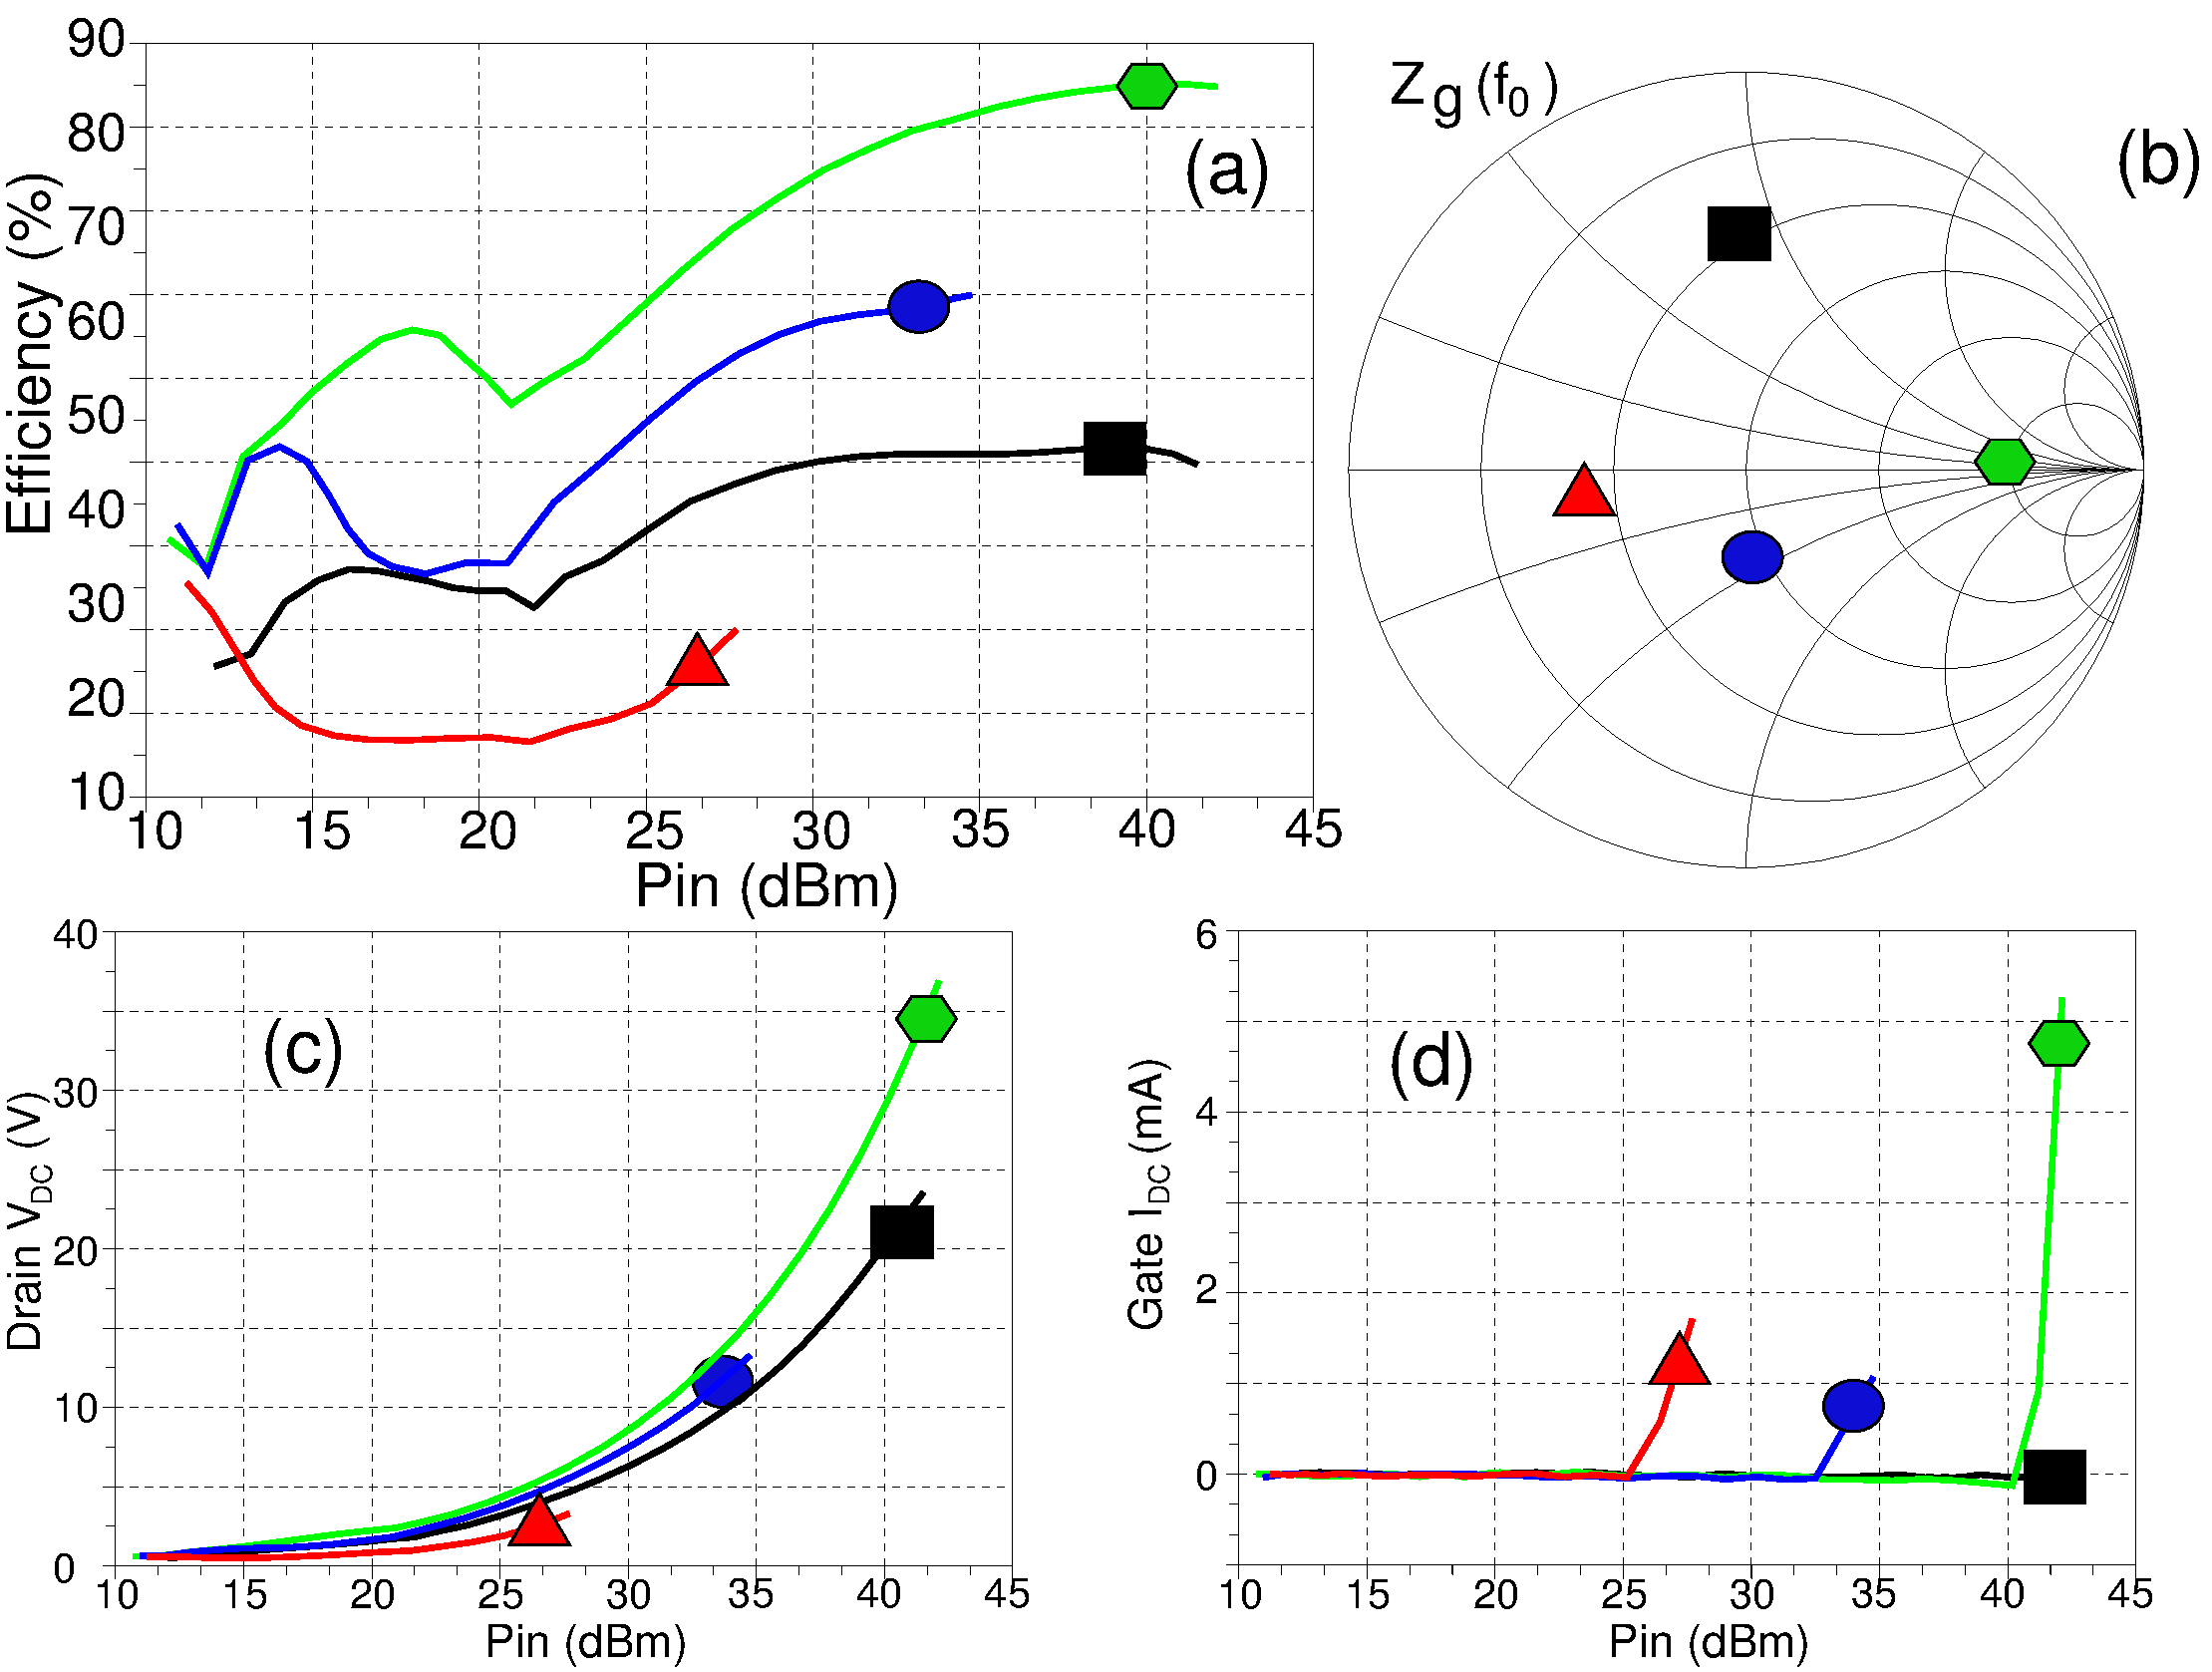
\includegraphics[width=3.4in]{pdf/12.pdf}
\caption{\hl{Conversion efficiency, gate DC current and drain DC voltage versus input power for several RF load impedance values presented at the gate. $V_{GS}=-4.4$\,V and $R_{DC}=98.5$\,$\Omega$. The green point on the Smith chart corresponds to the highest efficiency point at $Z_g(f_0)=\left(230+j10\right)\Omega$. }}
\label{MEAS_LP_sweep}
\end{figure}





% ===================================================================================================================================
% ===================================================================================================================================


%\subsubsection{Sweeping \textbf{Rd} - the resistance at the DC drain access}
After the optimal gate impedance for highest efficiency was obtained, a power sweep for three different $R_{DC}$ values in the drain output was obtained. From Fig.~\ref{Rd_sweep_final}, a maximal efficiency of 85\% was measured for a DC resistive load of 98\,$\Omega$ while an efficiency drop of 13\% was observed for a DC load of 21\,$\Omega$ with 40\,dBm input power. As expected, the DC output voltage decreases from a maximum \hl{30\,V} for $R_{DC}=98$\,$\Omega$ at 40\,dBm input power, to a maximum of 13.4\,V for $R_{DC}=21$\,$\Omega$ with the same input power. It is interesting to see how the input impedance of the rectifier at the RF drain port approaches 50\,$\Omega$ as the input power increases, Fig.~\ref{Rd_sweep_Zin}. This is expected, since the PA was designed for maximal saturated power delivered into a 50\,$\Omega$ load. This again points to the similarities between the same circuit operated as a power rectifier and a power amplifier.

% === FIG : Rd SWEEP
\begin{figure}[ht!]
\centering
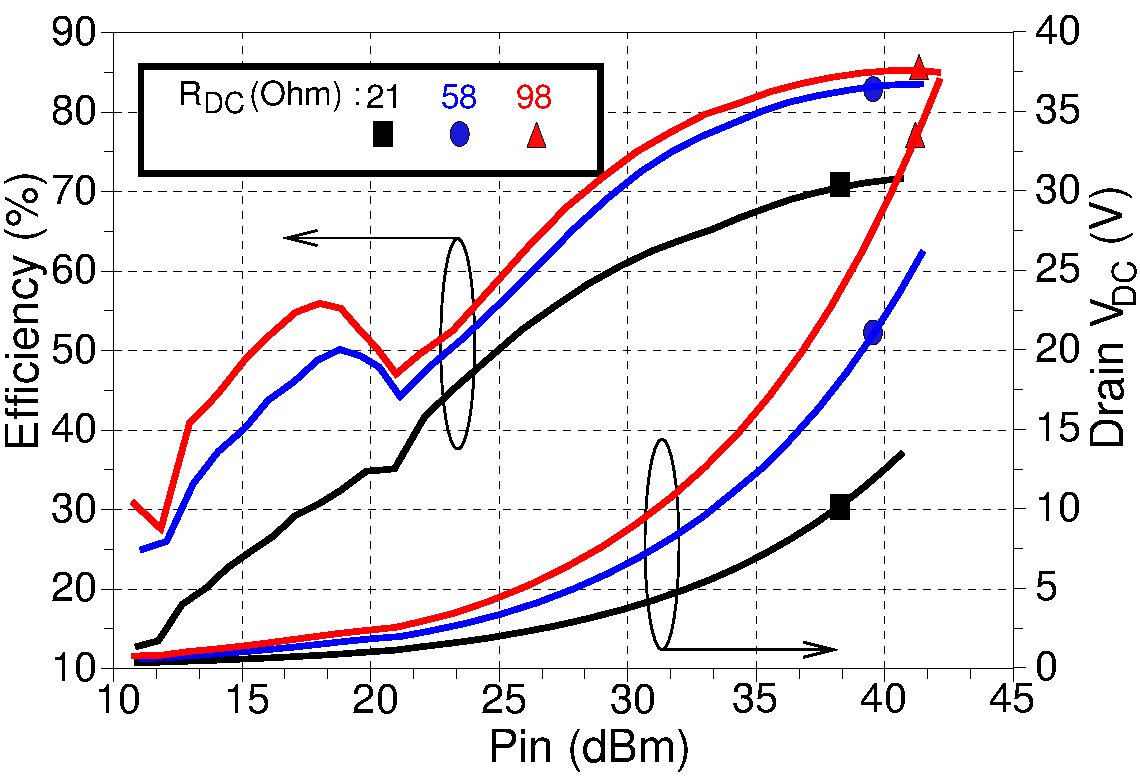
\includegraphics[width=3.4in]{pdf/13.pdf}
\caption{\hl{Conversion efficiency and drain DC output voltage versus input power for several DC drain resistor values. $V_{GS}=-4.4V$ and $Z_g(f_0)=\left(230+j10\right)\Omega$. The highest efficiency of 85\% is obtained at $P_{in}$=40\,dBm with a $V_{DC}$=30\,V.}}
\label{Rd_sweep_final}
\end{figure}


% === FIG : Zin
\begin{figure}[ht!]
\centering
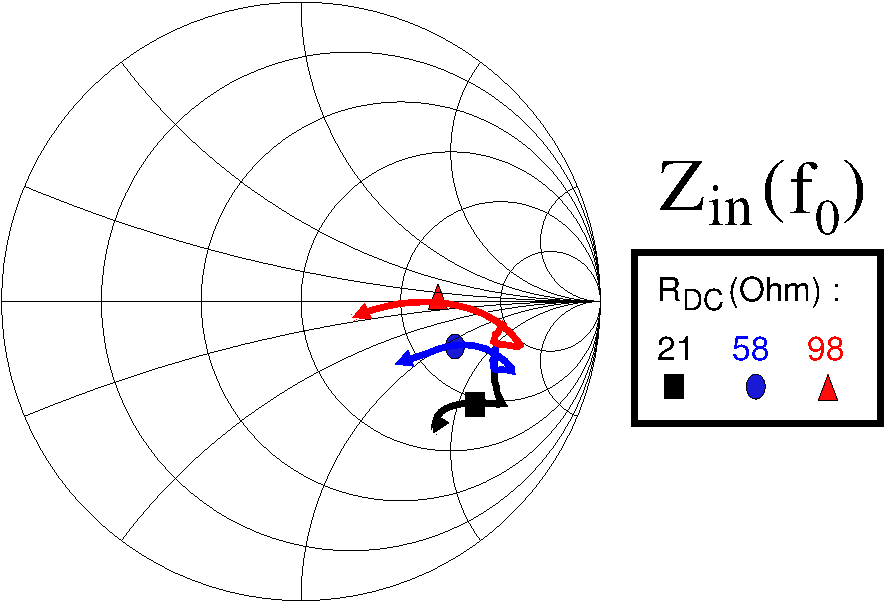
\includegraphics[width=3in]{pdf/14.pdf}
\caption{\hl{RF impedance at $f_0$ measured at the input (drain port) versus input power for several DC drain resistor values. $V_{GS}=-4.4V$ and $Z_g(f_0)=\left(230+j10\right)\Omega$.}}
\label{Rd_sweep_Zin}
\end{figure}



% ===================================================================================================================================
% ===================================================================================================================================
% \subsubsection{Sweeping \textbf{Vg} - the gate power supply}

Finally, the effect of the gate bias $V_{GS}$ on the rectifier efficiency, output voltage and input impedance was investigated. The gate impedance in this case was set for highest efficiency (230\,$\Omega$), and a DC load of 58\,$\Omega$ was selected in order to protect the transistor from high drain voltages that occur for the 98\,$\Omega$ load that corresponds to the highest efficiency. The measurements were performed for six different values of gate bias $V_{GS}$ as shown in Fig.~\ref{VG_sweep_final}. \hl{With $R_{DC}=58\Omega$,} a maximum efficiency of 83\% was obtained with the transistor biased deeply into the pinch-off region with $V_{GS}=-4.4$\,V, and a drop of only  3\% was measured for $V_{GS}=-3.5$\,V. Furthermore, the gate bias \hl{has a minimal impact} on the output DC voltage or on the drain impedance.


% === FIG : SWEEP VG
\begin{figure}[ht!]
\centering
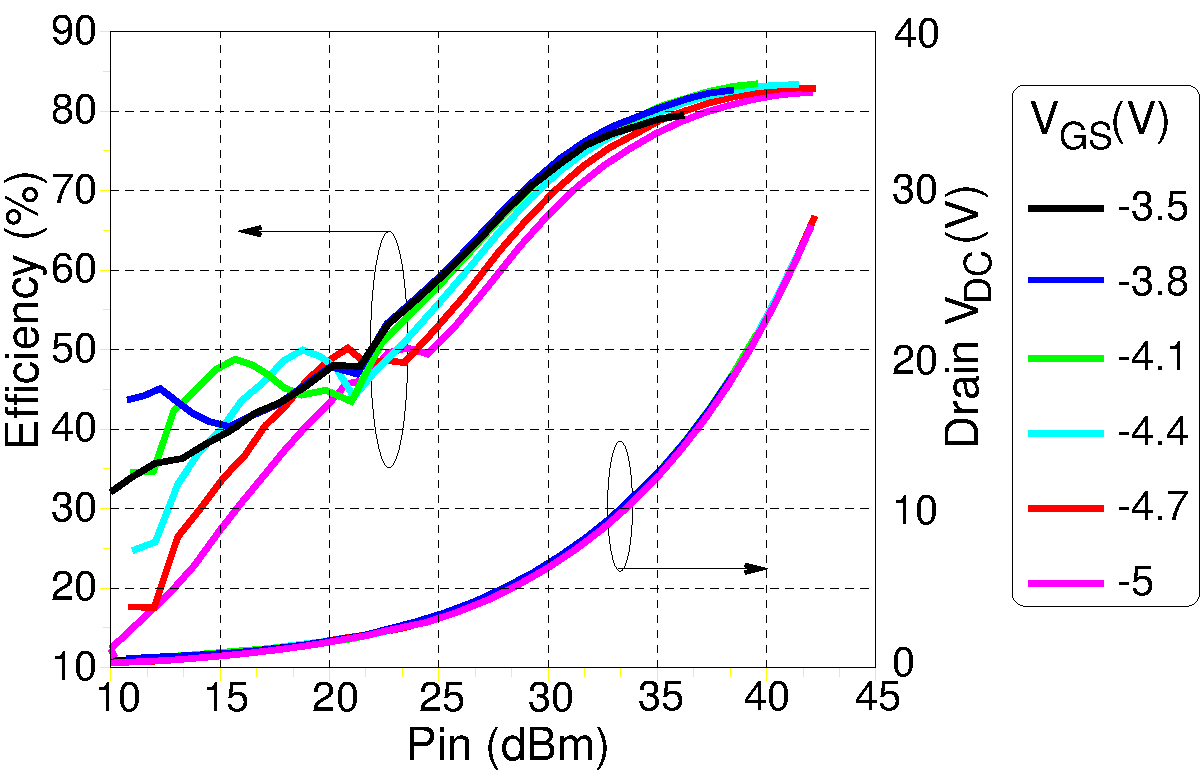
\includegraphics[width=3.4in]{pdf/15.pdf}
\caption{Measured conversion efficiency and drain DC voltage versus input power for several DC gate voltage biases. For this data, $R_{DC}=58\Omega$ and $Z_g(f_0)=\left(230+j10\right)\Omega$.}
\label{VG_sweep_final}
\end{figure}





% ===================================================================================================================================
% ===================================================================================================================================


% An example of a floating figure using the graphicx package.
% Note that \label must occur AFTER (or within) \caption.
% For figures, \caption should occur after the \includegraphics.
% Note that IEEEtran v1.7 and later has special internal code that
% is designed to preserve the operation of \label within \caption
% even when the captionsoff option is in effect. However, because
% of issues like this, it may be the safest practice to put all your
% \label just after \caption rather than within \caption{}.
%
% Reminder: the "draftcls" or "draftclsnofoot", not "draft", class
% option should be used if it is desired that the figures are to be
% displayed while in draft mode.
%
%\begin{figure}[!t]
%\centering
%\includegraphics[width=2.5in]{myfigure}
% where an .eps filename suffix will be assumed under latex,
% and a .pdf suffix will be assumed for pdflatex; or what has been declared
% via \DeclareGraphicsExtensions.
%\caption{Simulation Results}
%\label{fig_sim}
%\end{figure}

% Note that IEEE typically puts floats only at the top, even when this
% results in a large percentage of a column being occupied by floats.


% An example of a double column floating figure using two subfigures.
% (The subfig.sty package must be loaded for this to work.)
% The subfigure \label commands are set within each subfloat command, the
% \label for the overall figure must come after \caption.
% \hfil must be used as a separator to get equal spacing.
% The subfigure.sty package works much the same way, except \subfigure is
% used instead of \subfloat.
%
%\begin{figure*}[!t]
%\centerline{\subfloat[Case I]\includegraphics[width=2.5in]{subfigcase1}%
%\label{fig_first_case}}
%\hfil
%\subfloat[Case II]{\includegraphics[width=2.5in]{subfigcase2}%
%\label{fig_second_case}}}
%\caption{Simulation results}
%\label{fig_sim}
%\end{figure*}
%
% Note that often IEEE papers with subfigures do not employ subfigure
% captions (using the optional argument to \subfloat), but instead will
% reference/describe all of them (a), (b), etc., within the main caption.


% An example of a floating table. Note that, for IEEE style tables, the
% \caption command should come BEFORE the table. Table text will default to
% \footnotesize as IEEE normally uses this smaller font for tables.
% The \label must come after \caption as always.
%
%\begin{table}[!t]
%% increase table row spacing, adjust to taste
%\renewcommand{\arraystretch}{1.3}
% if using array.sty, it might be a good idea to tweak the value of
% \extrarowheight as needed to properly center the text within the cells
%\caption{An Example of a Table}
%\label{table_example}
%\centering
%% Some packages, such as MDW tools, offer better commands for making tables
%% than the plain LaTeX2e tabular which is used here.
%\begin{tabular}{|c||c|}
%\hline
%One & Two\\
%\hline
%Three & Four\\
%\hline
%\end{tabular}
%\end{table}


% Note that IEEE does not put floats in the very first column - or typically
% anywhere on the first page for that matter. Also, in-text middle ("here")
% positioning is not used. Most IEEE journals use top floats exclusively.
% Note that, LaTeX2e, unlike IEEE journals, places footnotes above bottom
% floats. This can be corrected via the \fnbelowfloat command of the
% stfloats package.



\section{Conclusion}
In summary, this paper addresses high-efficiency power rectifiers designed with harmonic terminations at the RF input, in analogy to high-efficiency power amplifier design with harmonic terminations at the output. The applications of such power rectifiers include wireless power beaming \cite{brown_rect2}, recycling power in high-power circuits \cite{asbeck} and ultra-fast switching integrated DC-DC converters with no magnetics \cite{4500dcdc}.

The theory for an ideal rectification element is based on Fourier analysis and establishes the basic design parameters such as the relationship between output DC resistance and impedance at the fundamental frequency at the rectifier input which optimizes efficiency. The analysis also predicts the time-domain waveforms at the terminals of the rectification element and the efficiency as a function of on-resistance and DC output resistance. Specific results are derived for class-C and class-F$^{-1}$ classes of operation, as they are defined for power amplifiers. These two cases are chosen for experimental validation with a 2.45\,GHz diode and 2.14\,GHz transistor rectifier, respectively. It is straightforward to repeat the derivation for other classes of operation, such as class-F as shown in detail in \cite{roberg_phd}.

The experimental results show that good agreement can be reached between theory and experiment with a Schottky-diode single-ended rectifier with finite class-C harmonic terminations, resulting in 72.8\% efficiency for input power levels in the mW range, intended for wireless power harvesting detailed in \cite{robergIMS2012,erezMTT2012}. A GaN pHEMT class-F$^{-1}$ power rectifier achieved 85\% efficiency with \hl{40}\,dBm input power across 98-\,$\Omega$ DC load \hl{with a DC output voltage $V_{DC}=30V$}. The efficiency and output voltage of the self-synchronous rectifier are shown to depend on the input power at the drain, the impedance at the gate port and the DC load at the output drain bias line, but not on the gate bias.

Time-domain large-signal measurements of a class-F$^{-1}$ power amplifier configured as a rectifier show that one can accomplish the same rectifier efficiency as the amplifier drain efficiency in self-synchronous mode without external gate RF drive. This is somewhat surprising, and to the best of our knowledge, the first time this type of high-efficiency rectifier has been demonstrated.



\section*{Acknowledgment}


%Dr. Reveryrand would like to acknowledge the funding by XLIM, Limoges, France.
The authors would like to thank Dr. David Root and Dr. Jean-Pierre Teyssier at Agilent Technologies for the loan of the time-domain nonlinear measurement equipment and TriQuint Semiconductor for the donation of the transistors.



% if have a single appendix:
%\appendix[Proof of the Zonklar Equations]
% or
%\appendix  % for no appendix heading
% do not use \section anymore after \appendix, only \section*
% is possibly needed

% use appendices with more than one appendix
% then use \section to start each appendix
% you must declare a \section before using any
% \subsection or using \label (\appendices by itself
% starts a section numbered zero.)
%

% ============================================
%\appendices
%\section{Proof of the First Zonklar Equation}
%Appendix one text goes here %\cite{Roberg2010}.

% you can choose not to have a title for an appendix
% if you want by leaving the argument blank
%\section{}
%Appendix two text goes here.


% use section* for acknowledgement
%\section*{Acknowledgment}


%The authors would like to thank D. Root for the loan of the SWAP. The SWAP that can ONLY be usefull in Boulder...


% Can use something like this to put references on a page
% by themselves when using endfloat and the captionsoff option.
\ifCLASSOPTIONcaptionsoff
  \newpage
\fi



% trigger a \newpage just before the given reference
% number - used to balance the columns on the last page
% adjust value as needed - may need to be readjusted if
% the document is modified later
%\IEEEtriggeratref{8}
% The "triggered" command can be changed if desired:
%\IEEEtriggercmd{\enlargethispage{-5in}}

% ====== REFERENCE SECTION

%\begin{thebibliography}{1}

% IEEEabrv,

\bibliographystyle{IEEEtran}
\bibliography{IEEEabrv,Bibliography}
%\end{thebibliography}
% biography section
%
% If you have an EPS/PDF photo (graphicx package needed) extra braces are
% needed around the contents of the optional argument to biography to prevent
% the LaTeX parser from getting confused when it sees the complicated
% \includegraphics command within an optional argument. (You could create
% your own custom macro containing the \includegraphics command to make things
% simpler here.)
%\begin{biography}[{\includegraphics[width=1in,height=1.25in,clip,keepaspectratio]{mshell}}]{Michael Shell}
% or if you just want to reserve a space for a photo:

% ==== SWITCH OFF the BIO for submission
% ==== SWITCH OFF the BIO for submission
\begin{IEEEbiography}[{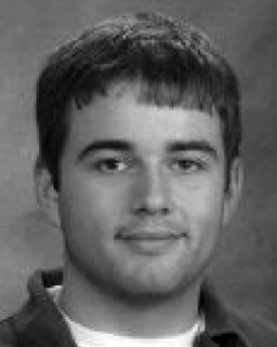
\includegraphics[width=1in,height=1.25in,clip,keepaspectratio]{photo/mike.png}}]{Michael Roberg}
(S'09) received the B.S.E.E degree from Bucknell University, Lewisburg, PA, in 2003, the M.S.E.E. degree from the University of Pennsylvania, Philadelphia, in 2006, and the Ph.D. degree from the University of Colorado at Boulder in 2012. From 2003 to 2009, he was an Engineer with Lockheed Martin–MS2, Moorestown, NJ, where he was involved with advanced phased-array radar systems. His current research interests include high efficiency microwave PA theory and design, microwave power rectifiers, MMIC design, and high-efficiency radar and communication system transmitters. He is currently employed by TriQuint Semiconductor - Defense Products and Foundry Services in Richardson, TX working on wideband high efficiency GaN MMIC PA design.
\end{IEEEbiography}
\begin{IEEEbiography}[{
\includegraphics[width=1in,height=1.25in,clip,keepaspectratio]{photo/tibo.png}}]{Tibault Reveyrand}
(M'07)  received the Ph.D. degree from the University of Limoges, France, in 2002.
From 2002 to 2004, he was a Post-Doctoral Scientist with CNES (French Space Agency). In 2005, he became a CNRS engineer at XLIM. His research interests include the characterization and modeling of RF and microwave nonlinear components and devices.
Dr. Reveyrand was the recipient of the 2002 European GaAs Best Paper Award and is a member of the IEEE MTT-11 "Microwave Measurements" Technical Committee.
\end{IEEEbiography}
\begin{IEEEbiography}[{
\includegraphics[width=1in,height=1.25in,clip,keepaspectratio]{photo/ignacio.png}}]{Ignacio Ramos}
(S'12) received the B.S. degree in electrical engineering from the University of Illinois at Chicago in 2009, and is currently working toward the Ph.D. degree at the University of Colorado at Boulder. From 2009 to 2011, he was with the Power and Electronic Systems Department at Raytheon IDS, Sudbury, MA. His research interests include high-efficiency microwave power amplifiers, microwave DC/DC converters, radar systems, and wireless power transmission.
\end{IEEEbiography}
\begin{IEEEbiography}[{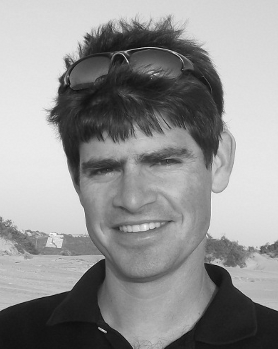
\includegraphics[width=1in,height=1.25in,clip,keepaspectratio]{photo/erez.png}}]{Erez Avigdor Falkenstein}
(S'07), Haifa, Israel in 1979. He earned a “Handesaie” degree (associate degree) in electronics from Amal Handesaim School Hadera, Israel in 1999. From 1999 to 2003 he served in the Israel Defense Force as part of a technological unit. He has been at the University of Colorado at Boulder 2004 – 2012. He received concurrent MS/BS degrees in Electrical engineering 2010 and a Ph.D 2012 from the University of Colorado at Boulder. Since 2007 he has been involved with research as part of the active antenna group. Research emphasis: far field wireless powering for low power densities. Interests include Antenna design and characterization, modeling and measurement of nonlinear devices at microwave frequencies and power management. He is currently employed at Qualcomm, Incorporated, Boulder, CO.
\end{IEEEbiography}
\begin{IEEEbiography}[{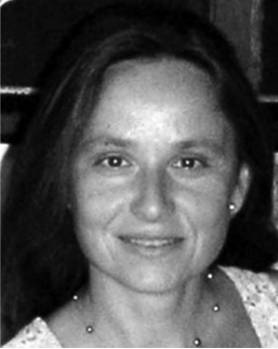
\includegraphics[width=1in,height=1.25in,clip,keepaspectratio]{photo/zoya.png}}]{Zoya Popovi\'c}
(S'86-M'90-SM'99-F'02) received the Dipl.Ing. degree from the University of Belgrade, Belgrade, Serbia, Yugoslavia, in 1985, and the Ph.D. degree from the California Institute of Technology, Pasadena, in 1990.
Since 1990, she has been with the University of Colorado at Boulder, where she is currently a Distinguished Professor and holds the Hudson Moore Jr. Chair with the Department of Electrical, Computer and Energy Engineering. In 2001, she was a Visiting Professor with the Technical University of Munich, Munich, Germany.
Since 1991, she has graduated 44 Ph.D. students. Her research interests include high-efficiency, low-noise, and broadband microwave and millimeter-wave circuits, quasi-optical millimeter-wave techniques, active
antenna arrays, and wireless powering for batteryless sensors.
Prof. Popovi\'c was the recipient of the 1993 and 2006 Microwave Prizes presented by the IEEE Microwave Theory and Techniques Society (IEEE MTT-S) for the best journal papers and the 1996 URSI Issac Koga Gold Medal. In 1997, Eta Kappa Nu students chose her as a Professor of the Year. She was the recipient of a 2000 Humboldt Research Award for Senior U.S. Scientists of the German Alexander von Humboldt Stiftung. She was elected a Foreign Member of the Serbian Academy of Sciences and Arts in 2006. She was also the recipient of the 2001 Hewlett-Packard (HP)/American Society for Engineering Education (ASEE) Terman Medal for combined teaching and research excellence.
\end{IEEEbiography}

%% if you will not have a photo at all:
%\begin{IEEEbiographynophoto}{Ignacio Ramos}
%(S'12) received the B.S. degree in electrical engineering from the University of Illinois at Chicago in 2009, and is currently working toward the Ph.D. degree at the University of Colorado at Boulder. From 2009 to 2011, he was with the Power and Electronic Systems Department at Raytheon IDS, Sudbury, MA. His research interests include high-efficiency microwave power amplifiers, microwave DC/DC converters, radar systems, and wireless power transmission.
%\end{IEEEbiographynophoto}

%% insert where needed to balance the two columns on the last page with
%% biographies
%%\newpage

%\begin{IEEEbiographynophoto}{Jane Doe}
%Biography text here.
%\end{IEEEbiographynophoto}
% ==== SWITCH OFF the BIO for submission
% ==== SWITCH OFF the BIO for submission



% You can push biographies down or up by placing
% a \vfill before or after them. The appropriate
% use of \vfill depends on what kind of text is
% on the last page and whether or not the columns
% are being equalized.

\vfill

% Can be used to pull up biographies so that the bottom of the last one
% is flush with the other column.
%\enlargethispage{-5in}



% that's all folks
\end{document}
